\documentclass[12pt, letterpaper, oneside, onecolumn]{report} % 
\author{William Baskin}
\title{Thesis}
\title{
  {A Biologically Inspired Controller for Efficient Trajectory Execution with Pneumatic Actuated Joints}\\
  {\large Case Western Reserve University \\
  Department of Mechanical and Aerospace Engineering}%\\
%	{\includegraphics{university.jpg}}
}
% \date{Day Month Year}
\date{\today}

\usepackage[utf8]{inputenc}
\usepackage[english]{babel}
\usepackage{csquotes}
\usepackage{graphicx}
\graphicspath{ {images/} }
% \includegraphics[height=6.75in,angle=270]{HW25}

\usepackage[margin=1in]{geometry}
\usepackage{setspace}
\doublespacing
\usepackage[style=ieee, backend=biber]{biblatex}
\addbibresource{references.bib}

\usepackage[hidelinks]{hyperref}
\usepackage{cleveref}

% https://tex.stackexchange.com/questions/119513/cleveref-and-appendix-packages-appendix-referenced-as-section
\crefname{appsec}{Appendix}{Appendices}

\newcommand{\myref}[1]{\hyperref[#1]{\Cref{#1}}}

%%% math %%%
\usepackage{amsmath, amssymb, amsthm}
\DeclareMathOperator*{\argmax}{arg\,max}
\DeclareMathOperator*{\argmin}{arg\,min}

% %%% Code %%%
% \usepackage{color}
% \usepackage{verbatim}
% \usepackage{listings}
% \definecolor{dkgreen}{rgb}{0,0.6,0}
% \definecolor{gray}{rgb}{0.5,0.5,0.5}
% \definecolor{mauve}{rgb}{0.58,0,0.82}

% \lstset{frame=tb,
%   language=Matlab,
%   aboveskip=3mm,
%   belowskip=3mm,
%   showstringspaces=false,
%   columns=flexible,
%   basicstyle={\small\ttfamily},
%   numbers=none,
%   numberstyle=\tiny\color{gray},
%   keywordstyle=\color{blue},
%   commentstyle=\color{dkgreen},
%   stringstyle=\color{mauve},
%   breaklines=true,
%   breakatwhitespace=true,
%   tabsize=3
% }


%%% Packages for the future %%%
% \usepackage{parskip}
% \usepackage{textcomp}
% \usepackage{soul}

\newcommand{\subsubsubsection}{\paragraph}
\newcommand{\bbs}[1]{\section{#1}}
\newcommand{\bbss}[1]{\subsection{#1}}
\newcommand{\bbsss}[1]{\subsubsection{#1}}
\newcommand{\bbssss}[1]{\subsubsubsection{#1}}

\newcommand{\norm}[1]{\left\lVert#1\right\rVert}

\begin{document}
\maketitle

% approval pdf

\tableofcontents

\listoffigures
% TODO(buckbaskin): verify that figures are the correct size, have axis labels, etc

\chapter*{Acknowledgments}
\label{chap:acknowledgements}
Acknowledged!

\chapter*{Abstract}
\label{chap:abstract}

This research develops a new synthetic nervous system for control of joints using pneumatic actuators in order to create a more efficient and adaptable walking robot system. This design implements new features not previously seen in a control oriented nervous system. It develops 3 major design components not previously used for control of antagonistic pneumatic actuators. It uses an internal model of the actuators to estimate the state of the joint. It uses internal estimates of the dynamics of the joint to continually optimize the control output. Additionally, it updates its own internal system model with a memory-like loop to allow the controller to adapt to any joint and trajectory. The controller allows for the replacement of proportional or other control designs with a learning system that decreases wasted antagonistic muscle activation and wasted energy, decreases phase lag and increases trajectory tracking accuracy.

\chapter{Introduction}
\label{chap:introduction}

Walking robots offer many advantages over wheeled robots or other types
of locomotion. Wheeled or tracked vehicles are unable to access over half
of the earth's landmass \cite{BigDog}. Further, many areas in which humans
operate are designed for walking as opposed to rolling, e.g. stairs, curbs or at a construction site, so a successful walking
robot would increase mobility in environments designed for human walking. On the
other hand, walking robots are harder to control than their wheeled
counterparts.

Many robot designers have looked to biological inspiration to increase the mobility and
ease of control of robots. In particular, many biological systems have increased
redundancy to aid in balance with many animals, including dogs and cats, walking
on 4 or more legs. The inspiration taken varies from imitating gait timing \cite{Raibert1986} to
help coordinate simple legs to completely mimicking musculoskeletal layout. The
Puppy robot (\myref{fig:Puppy}) was designed to mimic the operation of a large 
canine walking in the sagittal plane using pneumatic muscles and the \cite{PuppyDesign}.

Another advantage that animals have over most robots is their actuators.
Biological muscles are compliant and are a key part to how animals walk. Many
robots use electric motors or hydraulic actuators to actuate joints, which are stiffer than muscles and tendons, which can
mean that other biologically inspired design decisions cannot be applied directly. During the design of Puppy \cite[PuppyDesign], pneumatic artificial muscles were chosen, which have a higher
power to weight ratio than other designs and offer similar compliance and
behavior to biological muscles \cite{Tavakoli2008}. Pneumatic muscles have a unique design constraint: they only apply force during contraction. Therefore,
they are often used in antagonistic pairs. This is typically seen as a disadvantage because it increases the complexity of the robot; however, the muscles also allow for further bio-inspiration in the robot design
and control system.

One of the major trade offs for pneumatic muscles is that they exhibit
non-linear behavior in both static and dynamic control situations \cite{HuntPMuscles, DynamicPMuscles}. This has
motivated the designs of new types of controllers to overcome the non-linear
behavior through adaptation in the controller. In \cite{Jahanabadi2009}, the
authors propose a system called ``Active Force Control" where a neural network
is used to learn non-linear properties of the actuator and controlled mass.
The network is run in an inner control loop and the output of the network is
used to present the control situation in a linearized fashion to an outer PID
control system. The results suggest that a system model of the nonlinear
properties of the actuators decreases positional error. The work was
applied to controlling a vertical trolley and used a neural network as a black
box for modeling the system, so there is an opportunity to engineer a more transparent system that is easier to interpret and optimize for controlling Puppy's rotational joints.
In \cite{Wang2013}, a model-based controller was used to control the actuation
of a revolute joint with pneumatic muscles. The author's system allowed for
decreased antagonistic muscle overlap at high accelerations combined with a
high stiffness, high overlap controller for precise position tracking in near
static situations. This adapting system was shown to be effective in their
results; however, it does not account for estimating changing properties of the
robot system that might reduce the effectiveness of the model.

A combination of these two types of controllers offers insight into how to build
an effective joint controller for Puppy. One further area of potential
improvement over existing designs is the incorporation of biological inspiration
within the controller itself. In \cite{NickFunctionalSubnetwork}, the authors
demonstrate a method for using a dynamic, biologically accurate model of neurons
to develop models of neurons for controlling physical systems. The work in the
paper describes how to create building blocks such as arithmetic operations,
differentiation or integration. These components can then be used together to
recursively create new controller architectures that use biological inspiration
taken from literature for controlling legged robots and combine these components with an
efficient system for engineering the correct control responses. Together,
existing literature suggests that a neuron-based controller that adapts to the
properties of the muscles and the joints that it controls may offer a new
architecture for more efficient and more accurate control of pneumatic muscle-
actuated robots.

\section{Task Overview}

This thesis focuses on control of joints for the canine-inspired
Puppy robot in a walking scenario. The two distinguishing physical features of 
the robot are its pneumatic muscle actuators and a design that leans heavily
on the mechanics and skeleton of canines.

\begin{figure}
\centering
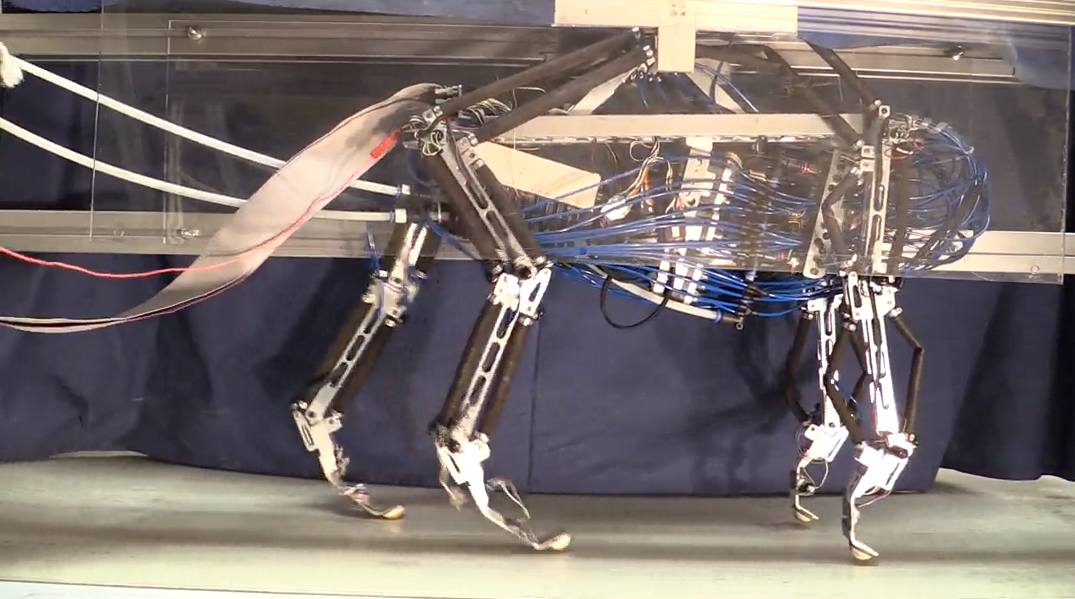
\includegraphics[width=5in]{introduction/Puppy}
\caption{The Puppy robot}
\label{fig:Puppy}
\end{figure}

\section{Specifications and Important Challenges}

There are a number of key criteria that are important for improving the behavior
of the joint controller. Based on previous work, these criteria break down as follows:

\begin{itemize}
\item Peak position during hip actuation is not accurate (5-15 deg) 
\item Delays between sensor data off the robot $\rightarrow$ lab view $\rightarrow$ Animatlab $\rightarrow$ lab
view $\rightarrow$ robot cause tracking problems
\item Scapula drives forward motion for front legs in the reverse Z orientation
\item Improve torque profiles to eliminate external support
\item Better internal understanding of dynamics to match desired and intended activation
\end{itemize}

These challenges drive three key requirements for the controller.

\begin{enumerate}
\item Decrease torque errors between neuron desired model and executed torques
\item Minimize phase shift between desired and achieved trajectory
\item Decrease position error during trajectory execution to less than 5 degrees from the desired position
\end{enumerate}

These challenges and requirements define two different components and desired
behaviors for the components within the controller. First, the controller should
incorporate an internal understanding of the dynamics of the joint. This will
allow for more optimized control. This also will allow for a model-based
approach where a few key parameters can be used to summarize the behavior of the
joint so that minimal example data can be used to finely tune the parameters and
model. Without an internal understanding of the dynamics, the controller would have to
use an arbitrarily complex neuron system to model an arbitrary behavior that may
over fit to the idiosyncrasies of a few data points and not generalize
effectively to continued modeling of the joint.

Second, the controller should perform internal optimization to provide an
improved output. There are multiple ways that this optimization can occur, but
an internal optimization step built into the controller will allow for the joint
to adapt and be more efficient across multiple behaviors where a simple
controller, such as a proportional controller, is statically tuned for a single
situation and will either be inefficient or inaccurate as the environment
changes. Each step on a walking robot is potentially different, so a static
controller will almost certainly be continually sub-optimal. A controller with a good internal model of the joint can use errors in past data to better fit the model to how the joint will behave and mitigate future error.

Additionally, an internally optimizing controller with a model of joint dynamics can
optimize for the estimated position of a joint at a time ahead of the current
sensor data. This means that, on a system with a known delay for sensor data
leaving the robot and control commands arriving at the robot, the controller can
control the robot as if it were already at the time in the future where the
joint will be instead of at the point in the past where the joint was when the
sensor data was read.

\section{This Work}

This work continues with a review of surrounding and supporting literature in 
\myref{chap:lit_review}. \myref{chap:controller_design} discusses the design of 
a internal model adaptive controller that incorporates the design goals of 
understanding the dynamics, projecting forward in time and optimizing the 
controlled output based on the understanding of dynamics. \myref{chap:neuron_design} discusses the implementation of the controller within a 
synthetic nervous system simulation. This discussion talks about some 
simplifications and approximations that were made in the process, as well as 
areas of the network that are more complex improvements over the controller 
design discussed in \myref{chap:controller_design}. \myref{chap:methods} 
discusses the methods used to design, iterate, test and validate the controller 
designs. \myref{chap:results} discusses the results of testing the controllers.
\myref{chap:conclusion} discusses the conclusions and future work.


\chapter{Literature Review/Background}
\label{chap:lit_review}
\bbs{Puppy}

The canine-inspired robot Puppy was designed to prove the feasibility of using
pneumatic muscles for actuating a quadruped robot. The design focuses on 
imitating the musculoskeletal parameters of an adult greyhound 
\cite{PuppyDesign}. This work is motivated by extensions and potential
improvements to a control method developed by Alex Hunt in
\cite{HuntPhDThesis} and \cite{HuntHindLegWalking}. Among other areas identified
for improvement and future work, the Hunt thesis in particular cites accurate torque
profiles as a key improvement for increasing the stability and mobility of the
robot. Related to the accurate torque profiles, the joint peak angles are
accurate to between 5 and 15 degrees, but further improving the accuracy offers
an avenue for more effective walking. One potential source of error in the
hardware system is the delay between a sensor reading, communicating the data to
an off-board computer and then communicating a command back to the robot. The end
result of the current Puppy control system is that the hind legs can walk effectively;
however, the front legs can trip or otherwise get stuck under the body of the
robot.

\bbs{Similar Robots}

There have been multiple variations of walking robots in 2-legged and 4-legged
configurations. Canines and felines are a common inspiration for these kinds of
robots, with inspiration ranging from very low degree of freedom (single joint
per leg) robots that mimic gait timing to robots that attempt to implement
complete structural and muscular replications of dogs or cats.

\bbss{Canine Robots}

The Big Dog robot made by Boston Dynamics (along with the more recent Spot and
Spot Mini) are quadruped robots built specifically for enhanced all terrain
mobility. According to \cite{BigDog}, less than half of land terrain is
accessible to wheeled or tracked vehicles, so legged robots have the opportunity
to offer unparalleled mobility.

The robot ``Ken" is based on canine kinematics with a focus on designing for
high frequency operation. The design is focused on being lightweight while also
being biomimetic. One key design decision was the use of pneumatic muscles over
electric motors. This facilitates high speed and high frequency operation
without the typical heating and/or cooling issues. Another interesting design
decision for the Ken robot was the incorporation of a contractor muscle at the
hip. Its placement and operation shorten or lengthen the leg mechanism
independent of the flexion or extension of the leg \cite{Narioka2012}.

\bbsss{Dynamics of Canine Robots}

The dynamics of robots, even those that attempt to accurately mimic biological
mechanisms, can vary significantly in performance from their biological
counterparts. For example, mirroring the standard Z configuration of a canine-
inspired robot can actually increase its efficiency by better utilizing passive
spring elements. This suggests that animals may have adapted gaits and
stimulation patterns for redundant muscles that take better advantage of passive
properties of muscles than are accommodated for in current control designs \cite{HindLegMorphology}.

Passive elements and the particular properties of a joint play a strong role in
the energy required to actuate the joint and the effective frequency at which the joint
can operate. In particular, \cite{Na2015} covers the design of a spring
mechanism with a high natural frequency to increase the amplitude of joint
motion during high frequency operation.

\bbss{Other Robots with Pneumatic Muscles}

% TODO(buckbaskin): insert a photo of pneumatic air muscles, one relaxed and one pressurized

In \cite{PAMApplicationSurvey}, many biorobotic applications for pneumatic
muscles are presented.
Additionally, the devices are used for medical applications where the an actuator's
inherent compliance, lighter weight and higher power output are also important. 

The Pneupard robot is a feline-inspired robot based on a cheetah's
musculoskeletal design. It is actuated using pneumatic muscles to control each 3
degree of freedom leg. To control the leg, a rules-based controller is used to switch between
states where muscle activation in an actual cat are mapped to pressures in each
muscle. This controller design was aided by taking a biomimetic approach to determining the lever
arms by which the pneumatic muscles actuate. The results showed that the simple
control system remained effective even in the face of obstacles in the robot's
path due to the compliant biomechanical design \cite{Pneupard2013}.

In \cite{Wait2014}, the authors show that a simpler controller design can be
used on a quadruped robot with biologically inspired design to achieve a highly
power dense design that walks effectively. The control approach focuses on
a high-impedance control scheme for the stance phase and a second state
that takes advantage of pneumatic actuator compliance during the swing phase.
This design does not use pneumatic muscles. Instead, the authors use pneumatic
cylinders to make the design more compact by using a single rigid pneumatic cylinder that can apply both
flexion and extension forces on a joint. 

\bbs{Pneumatic Actuators}

Pneumatic artificial muscles typically consist of a high pressure source, a
flexible polymer section and an exhaust valve. The muscle contracts in length
when the internal pressure is higher than the surrounding environment. During
this contraction, the muscle applies a force. One limitation of pneumatic
muscles is that they typically are unable to apply force during relaxation in
the same way a rigid pneumatic cylinder can. Instead, pneumatic muscles typically are used in
antagonistic pairs. The nonlinear nature of the pneumatic muscles combined with the
antagonistic design means that, in practice, simple linear controllers are
ineffective at accurately executing a trajectory with pneumatic muscles. This means that more complex controllers are required; however,
this also means that the controller design can be more tailored and take
advantage of the unique properties of two antagonistic nonlinear actuators.

Pneumatic actuators are less common in robotics compared with electric motors;
however,
they often result in a lighter system for controlling a joint than an
electric motor. There are trade offs to each, but pneumatic actuators offer a
higher power to weight ratio for smaller displacement at low velocity and
often are a significant improvement over electric motors at higher velocities \cite{Tavakoli2008}. These properties suggests that pneumatic muscles are well suited for applications in
biological walking robots where an increased power to weight ratio increases
the efficiency of the walking mechanism, especially at the high joint velocities
found in a stepping motion.

\bbss{Characterizing Pneumatic Actuators}

In \cite{Situm2008}, the authors analyze gas flow properties for fluidic muscles
and experimentally quantify the performance of the pneumatic muscles in an antagonistic coupling
through a pulley. One of the key conclusions in \cite{Situm2008} motivating future work is the
demonstration for a single joint with most external factors removed. The
proportional-integral control as implemented was unable to fully correct for
errors even in a desired trajectory composed of slow steps to a constant value
where the control system had time to reach a set actuation pressure.

Pneumatic actuators are used on the Puppy robot. One of the key
benefits of using pneumatic muscles in a biologically-inspired robot design is
that the muscles have similar properties to the biological muscles that control
canines \cite{Tavakoli2008}.
During analysis of the behavior of pneumatic muscles with a static load, the muscles demonstrated a non-linear response to
changing length and the ability to apply a force. This relationship was
quantified and generalized in \cite{HuntPMuscles}. This research showed that
there is a relationship between the strain on the muscle and the pressure
required to support a fixed load that can be approximated by a shifted tangent
function. 

\begin{figure}[h!]
\centering
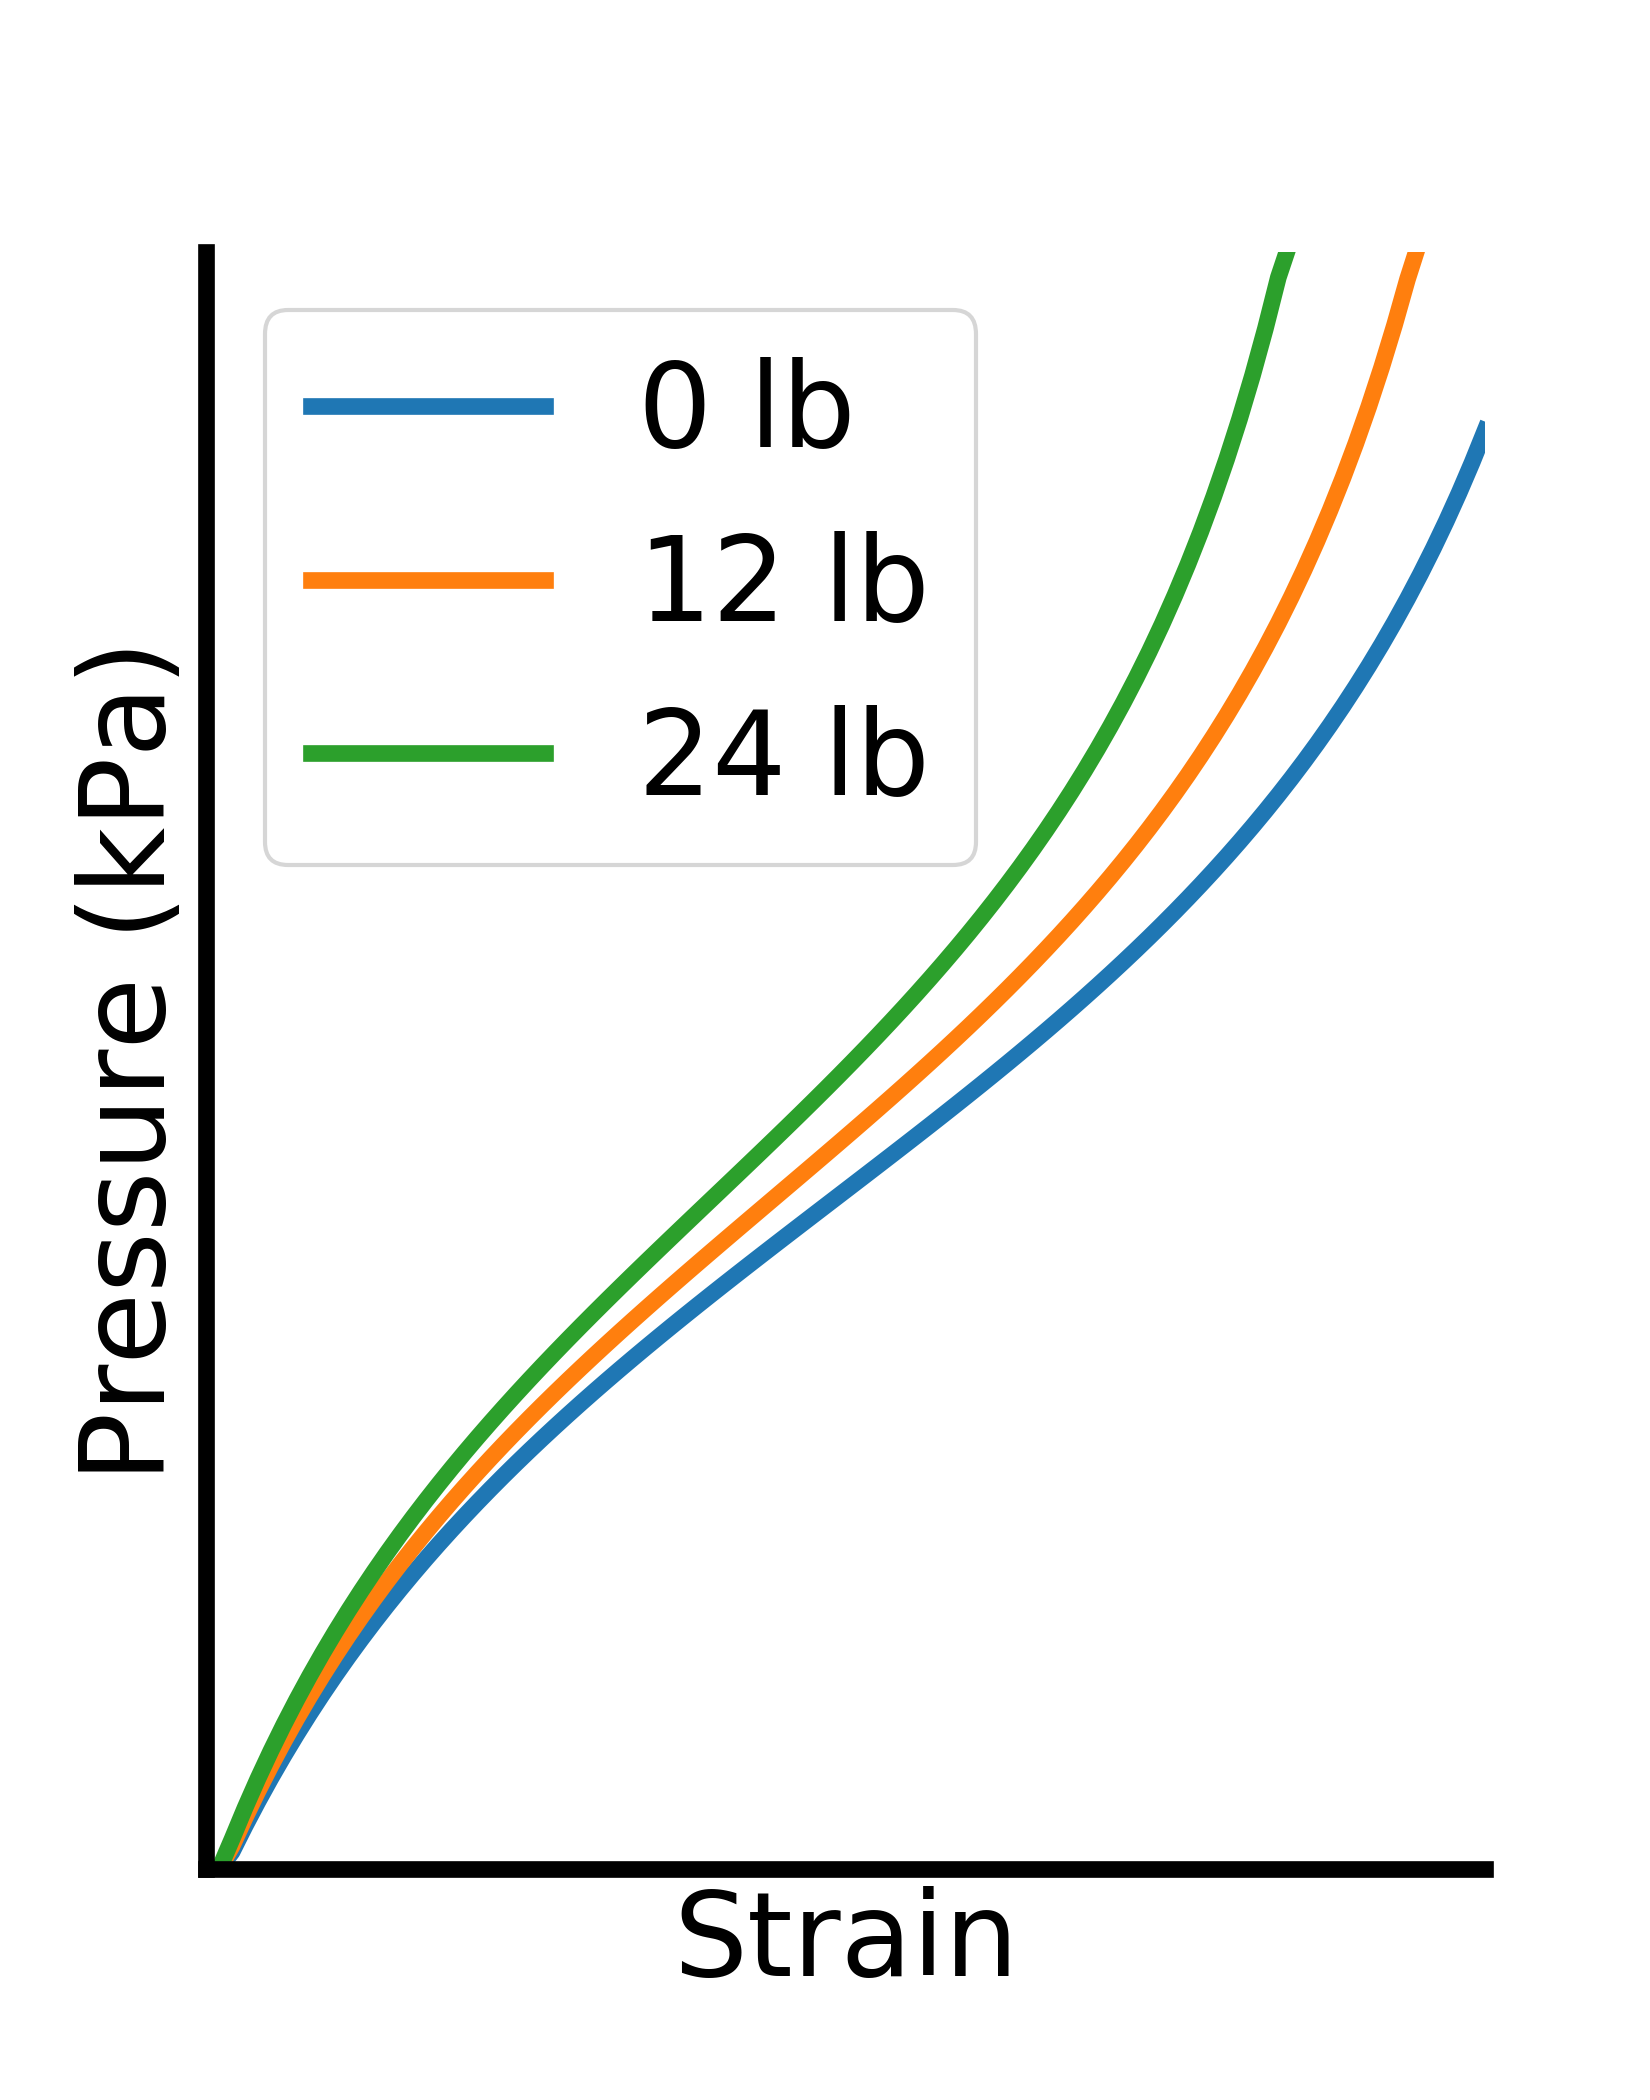
\includegraphics[width=5in]{lit_review/FigStrainPressure}
\caption{Strain/pressure relations for different applied loads}
\label{fig:StrainPressure}
\end{figure}

Using test and validation sets, the model was fit to data collected
from existing actuators on Puppy. Further, the paper goes on to show that the
model helps derive a controller for semi-static motion of joints \cite{HuntPMuscles}.

Other research with pneumatic muscles provides a model for incorporating the
dynamic properties of pneumatic actuators to allow for a more fine tuned control
process. In \cite{DynamicPMuscles}, the authors use dynamic application and
removal of load to measure the effective spring constant of the muscles and the
effective damping constant. The spring constant was shown to be correlated with
pressure, with a small constant spring effect at no pressure from the muscle
material itself. The damping coefficient was shown to be positively correlated
with pressure during contraction and weakly negatively correlated with pressure
during relaxation. The work suggests that damping comes from internal
friction in the actuator design. Additionally, the damping due to friction
effects in the input and exhaust lines is shown to be minimal compared to
internal actuator effects \cite{DynamicPMuscles}.

\bbs{Controller Design}

\bbss{Controller Theory}

Revolute joint position controllers can be treated as a function mapping the current
state (typically position, velocity and acceleration) to a torque to match the 
desired trajectory, expressed as position but often constrained to be a twice
differentiable function.

\begin{equation}
M(\theta) \ddot{\theta} + C(\theta, \dot{\theta}) \dot{\theta} + N(\theta, \dot{\theta}) = \tau
\end{equation}

If the robot starts at its desired initial state and the model of the robot is
perfectly known, the robot will exactly track the trajectory. Feedback in the 
form of sensory input is used to correct for starting error or error in the 
formulation of the exact model.

One common formulation for control is a proportional-derivative controller, 
where torque is chosen as the following:

\begin{equation}
\tau = -K_{v} \dot{e} - K_{p} e
\end{equation}

where

\begin{equation}
e = \theta - \theta_{d}
\end{equation}

The proportional-derivative (PD) controller results in a system that is stable, but does not converge to
exact tracking for most real systems. In practice, an integral term is often added that accounts for steady state error to create a proportional-integral-derivative (PID) controller; however, the additional of an integral term can lead to windup or other issues.

One general method for overcoming these limitations is to use a model of the 
system to perform what is known as computed torque control, where the actuator
applies enough torque to account for the $C(\theta, \dot{\theta})$ and
$N(\theta, \dot{\theta})$ terms and then applies the desired acceleration. This feed-forward term is written as follows:

\begin{equation}
\tau = M(\theta) \ddot{\theta_{d}} + C(\theta, \dot{\theta}) \dot{\theta} + N(\theta, \dot{\theta})
\end{equation}

To correct for initial error or otherwise, additional proportional terms are
added to the acceleration term:

\begin{equation}
\tau = M(\theta) (\ddot{\theta_{d}} - K_{v} \dot{e} - K_{p} e) + C(\theta, \dot{\theta}) \dot{\theta} + N(\theta, \dot{\theta})
\end{equation}

These additional terms are known as the feedback component. Since these 
corrections are linear in a system that is linearized by the feed-forward term,
values for the gains easily can be chosen to make the system stable and converge
to exactly following the desired trajectory (i.e., make the system exponentially stable) \cite{MLS94}.

Control via computed torque 
is not always practical because it requires the system to have a good model of 
itself with known parameters that incorporate many potential variations of the
system. In practice, 
there are many different ways to achieve effective control for a rotational 
joint.

\bbss{Revolute Joint Position Controllers}

In \cite{EventBasedWalking}, a new controller paradigm is proposed where control
is done by switching between known phases in a state machine based on sensory
events to generate an adaptable trajectory similar to purely time-based
trajectories where stability was achieved by a separate stability adjustment
system. Work in \cite{EventBasedWalking} focuses on control of a biped robot; however, the lessons can
be applied to a quadruped.

Event-based control through reflexes was also proposed as a way for additional
improvement of the existing synthetic nervous system in \cite{HuntPhDThesis}.
The Hunt thesis \cite{HuntPhDThesis} suggests that a particular a reflex known as the elevator reflex,
where the paw strikes an
obstacle mid-swing, could be used as the design inspiration for an internal recovery
mechanism to prevent tripping.

\bbss{Controllers for Pneumatic Muscles}

Multiple different methods have been proposed specifically for controlling 
pneumatic muscles.

In \cite{Jahanabadi2009}, the authors use Active Force Control
to control a pneumatic muscle for a prismatic joint. The system was designed to
use a PID control system as an outer loop with an inner loop based around an
artificial neural network to adapt to disturbances and other dynamic phenomena.
In practice, the system used a neural network to learn the nonlinear parameters
seen in the feed-forward term of the computed torque controller to provide a
nearly linear system to the PID controller. This system used a very simple
artificial neuron network to learn the system model, which is approximated as an
effective mass. The results of the paper show that the PID controller alone did
not track a square or saw-tooth wave well, and the system was improved by
incorporating a nonlinear system model. This work suggests that a pneumatic 
muscle system with a controller that has a good system model can be effective; however, the performance can be further improved with a better model of the
actuator itself and tailoring the controller to a robotic application as opposed
to a vertical trolley.

In \cite{Wang2013}, the authors discuss using a model based control method that
attempts to minimize the antagonistic muscle activation during operation in
order to better track a trajectory and imitate the muscle activation of a
biological system. The end result was the merger of both a high stiffness 
controller for operation near the desired trajectory and a high torque system
for high velocity or large error corrections. This work suggests that a system 
that smoothly combines these two behaviors will be highly effective, measured by
joint tracking accuracy for a steady position, joint tracking at high 
acceleration and velocity as well as joint efficiency and reduced antagonistic
waste. On the other hand, this model based system does not appear to estimate
parameters of the system that can continually change, which opens up an avenue
for potential improvement.

\bbs{Similar Neurons}

Neuron-based controllers offer a wide range of benefits over typical controller
designs. Neurons offer a dynamic way to represent control calculations that can
update and adapt to edge cases and perturbations in a system in a consistent 
way. Additionally, insights from biological nervous systems can be used to 
directly improve the performance of controllers, especially those controlling 
bioinspired systems. There have been issues with understanding how
to tune these neuron networks; however, as presented in 
\cite{NickFunctionalSubnetwork}, the neuron models can be adapted with 
relatively few parameters to replicate arithmetic and calculus operations, 
opening the door for an engineering approach to constructing and optimizing a synthetic nervous system.

\bbss{CPGs}

Many neuron control systems for oscillating joints incorporate central pattern
generators (CPGs), including 
\cite{Narioka2012, EventBasedWalking, HuntHindLegWalking, HuntPhDThesis}.
In their most reduced form, CPGs are a small bundle of
neurons that oscillate continually without requiring outside stimulation. They
have been implemented in multiple ways, but the underlying principles and 
biological motivation remain the same \cite{CPGReview}.
In
practice, CPGs often are connected to muscles through pattern formation or other
layers to convert the CPG cycle into muscle activation instead of directly
activating motor neurons. The pattern formation neurons are designed with a variety of topologies. Together with the CPG neurons they are grouped into single-level,
single-plus-level or two-level CPG models \cite{MultiLevelCPG}.

In insects and other animals, CPGs have been shown to combine with peripheral 
sensory feedback and
descending signals to coordinate walking motion between multiple joints and
limbs. The effects of sensory input come into the system as resetting or non-resetting deletions
along with other sensory effects that synchronize the oscillation of the CPG
with other limbs or mechanical motion, even in a decerebrated animal
\cite{SixLeggedWalking, CPGReview}.

\bbss{Neuron Design}

Neuron-based controllers often are designed in a data-driven way, where the
neuron system is treated as a black box. Recent work, collected in 
\cite{NickFunctionalSubnetwork}, shows that a more detailed neuron model can be
used to build up small subnetworks of neurons that perform a specific task,
including arithmetic operations like addition, subtraction, multiplication and
division, as well as operations such as integration and differentiation.

\begin{figure}
\centering
\begin{tabular}{cc}
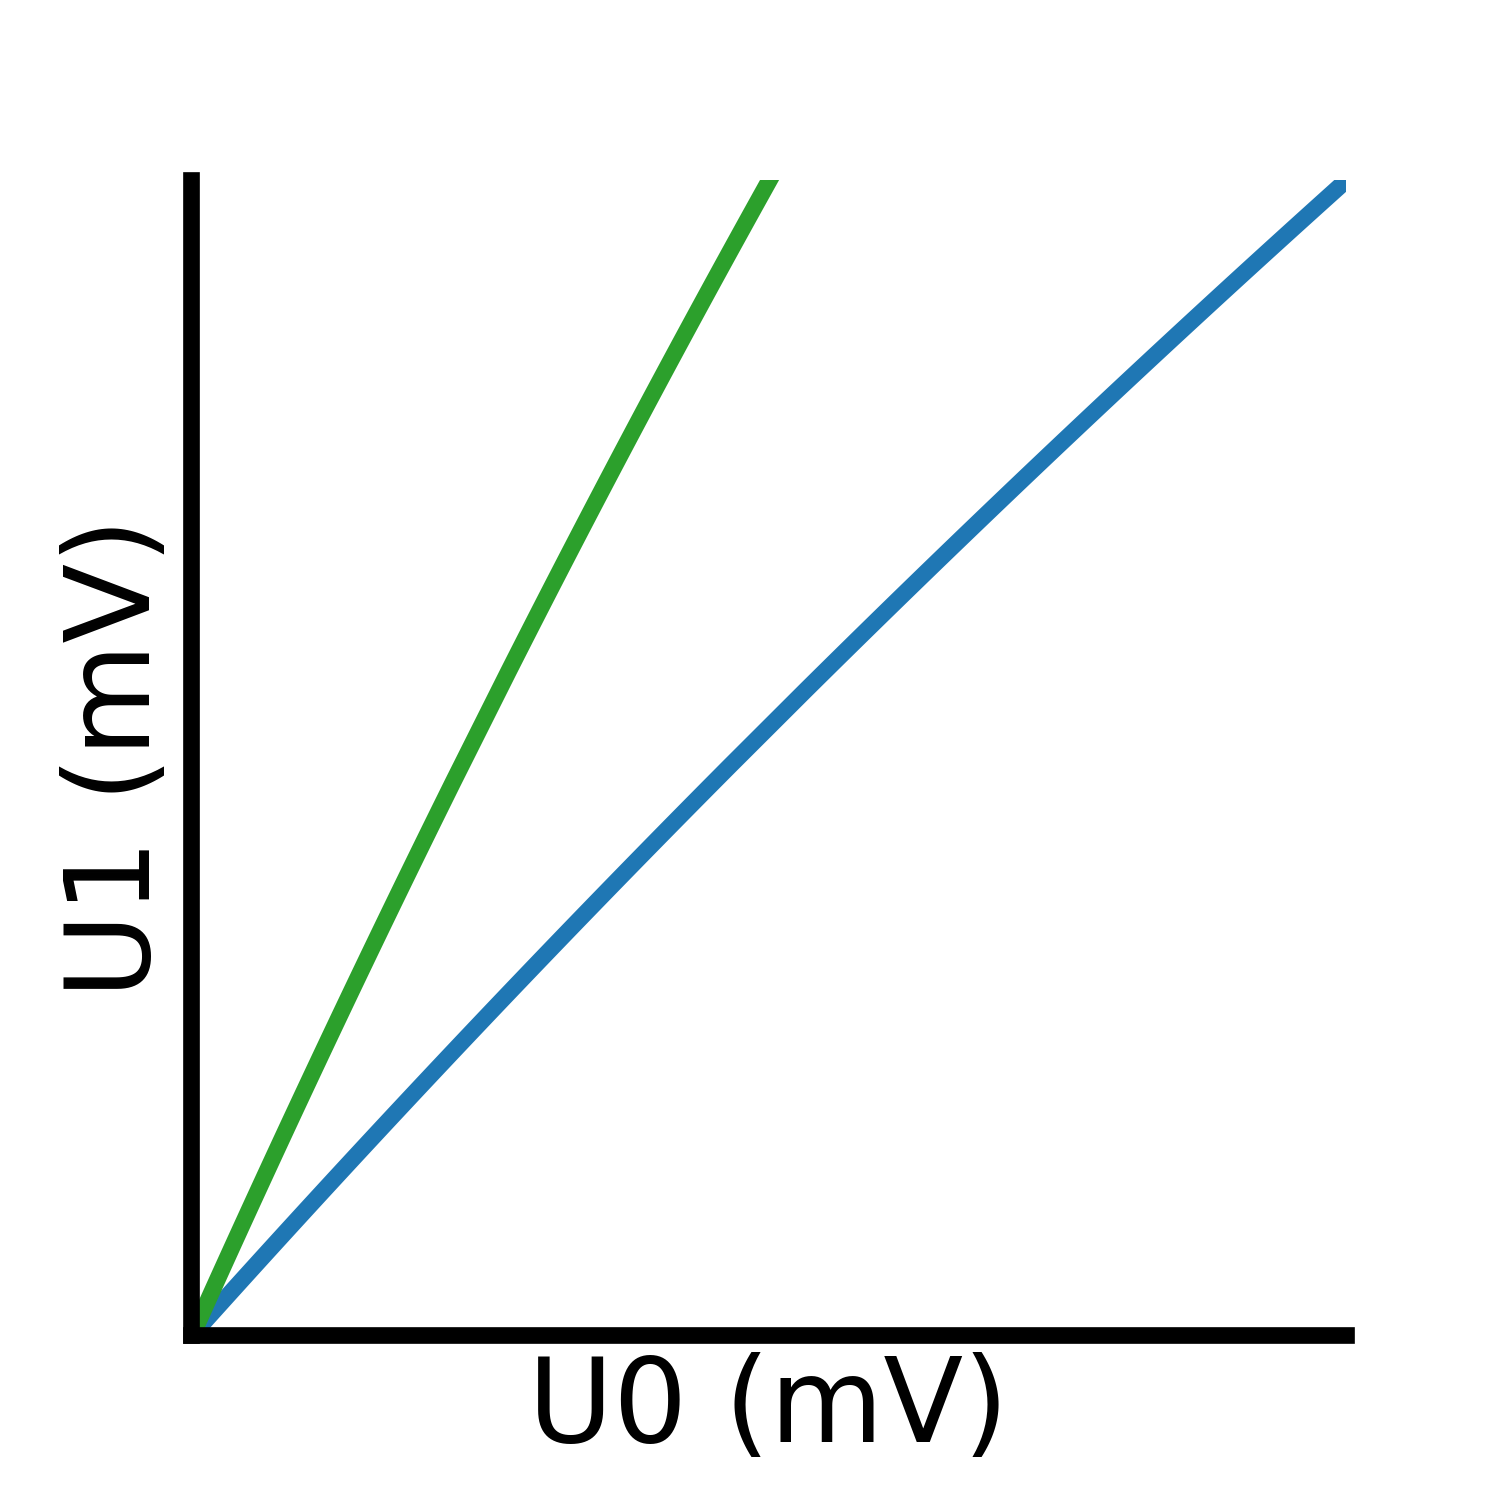
\includegraphics[width=3in]{lit_review/FigAdd} &
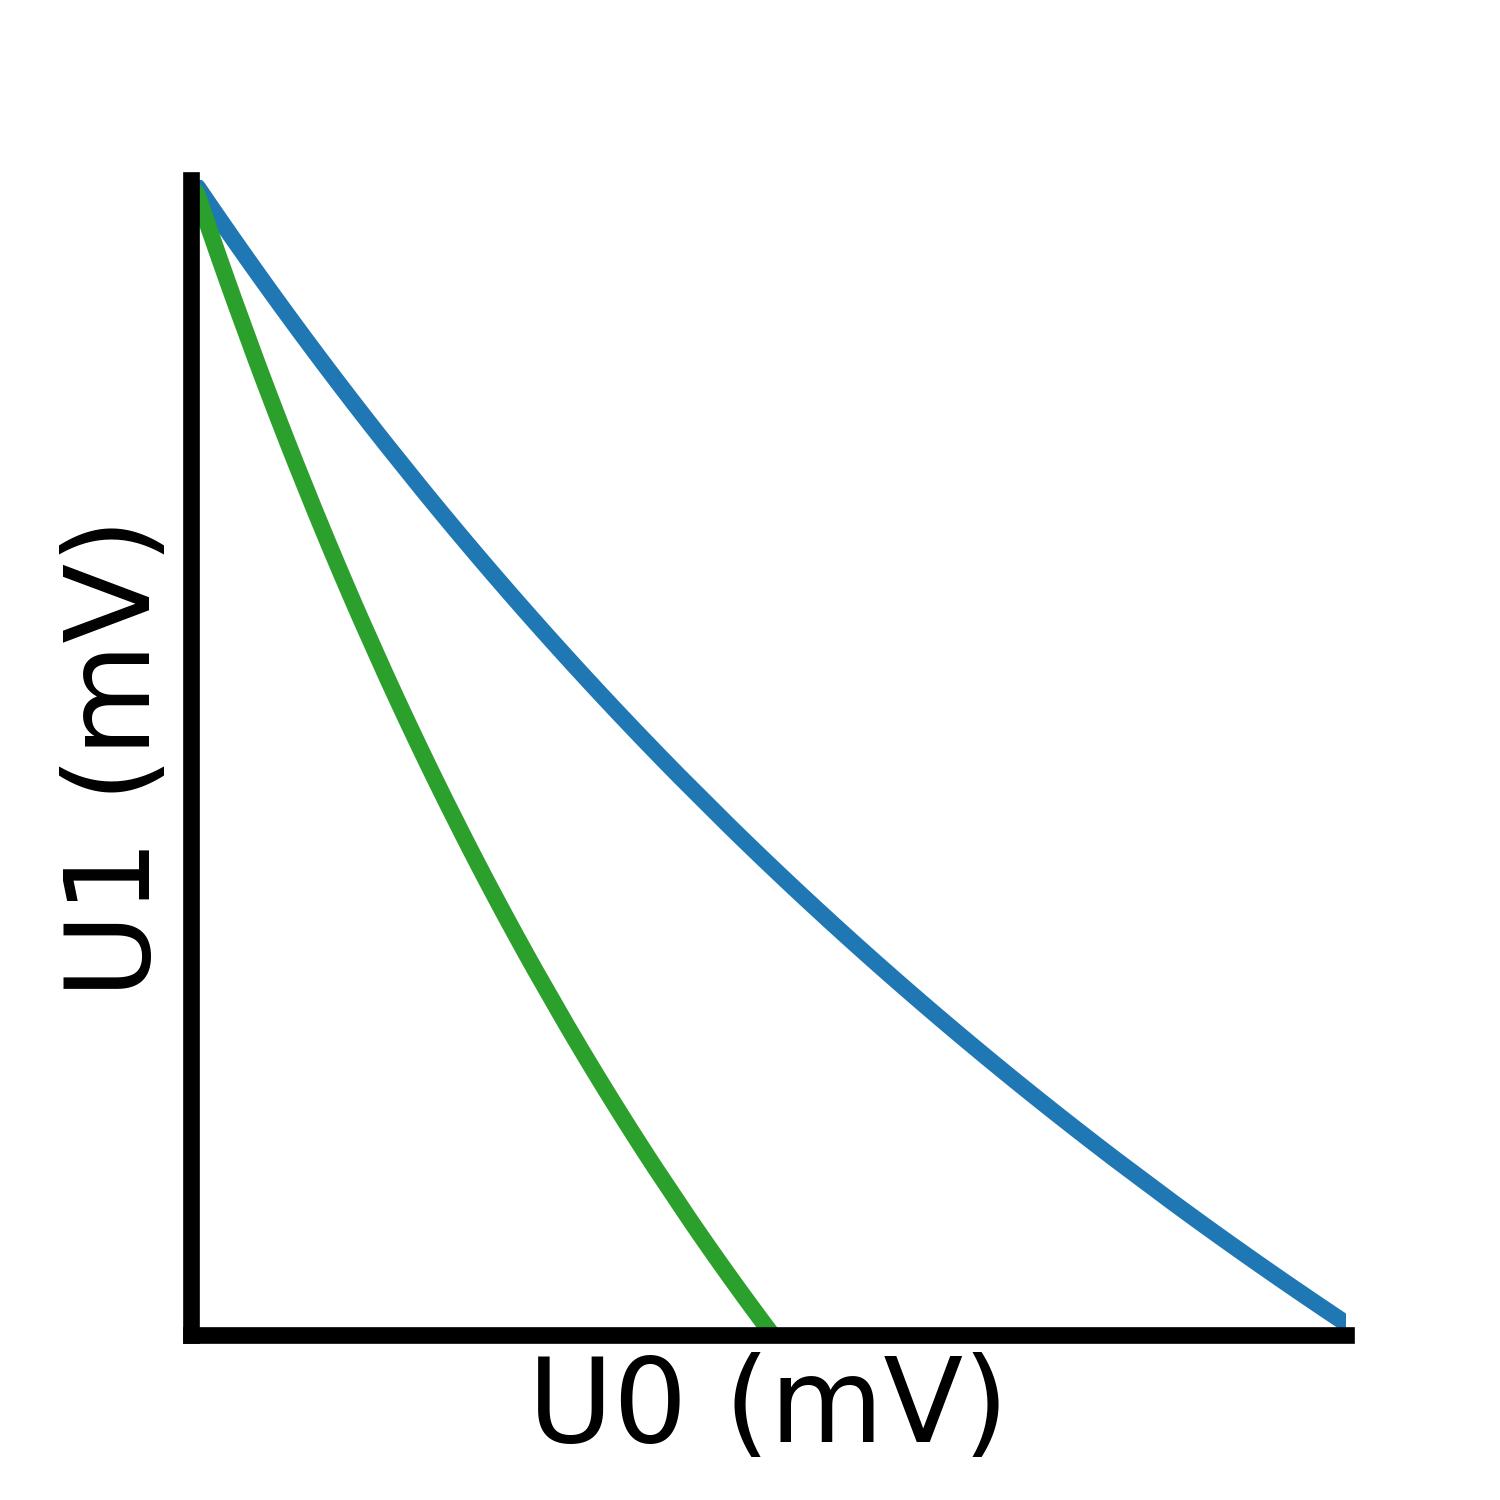
\includegraphics[width=3in]{lit_review/FigSub} \\
(a) Addition & (b) Subtraction \\
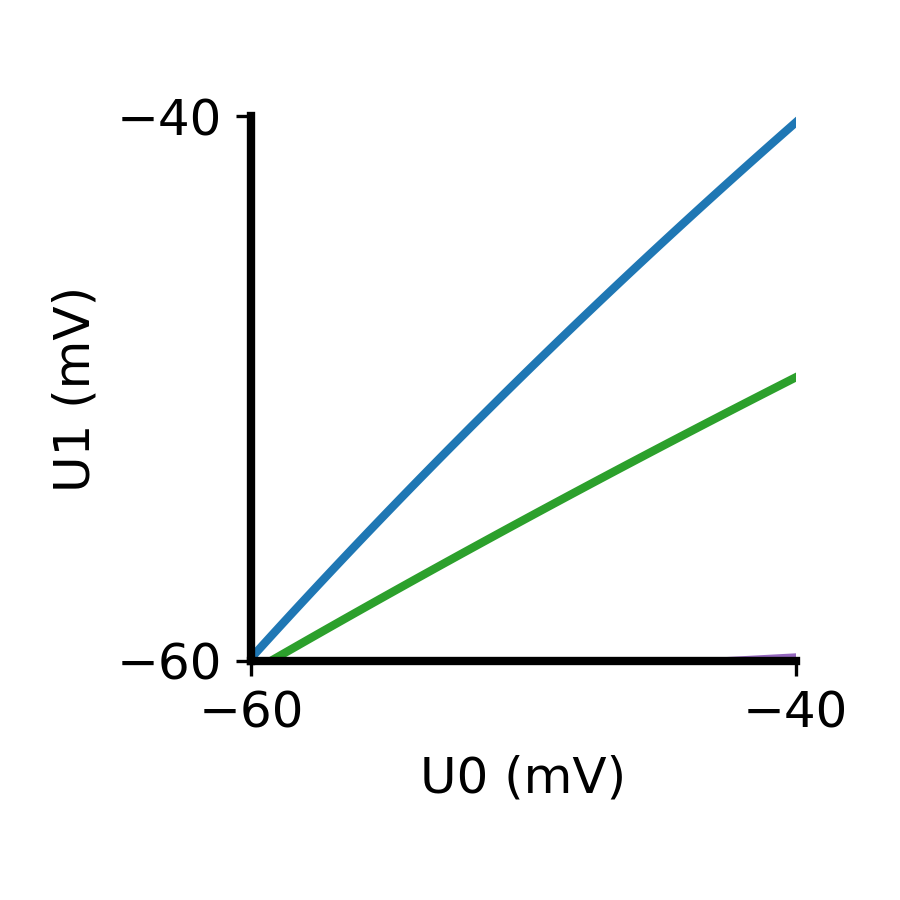
\includegraphics[width=3in]{lit_review/FigMul} &
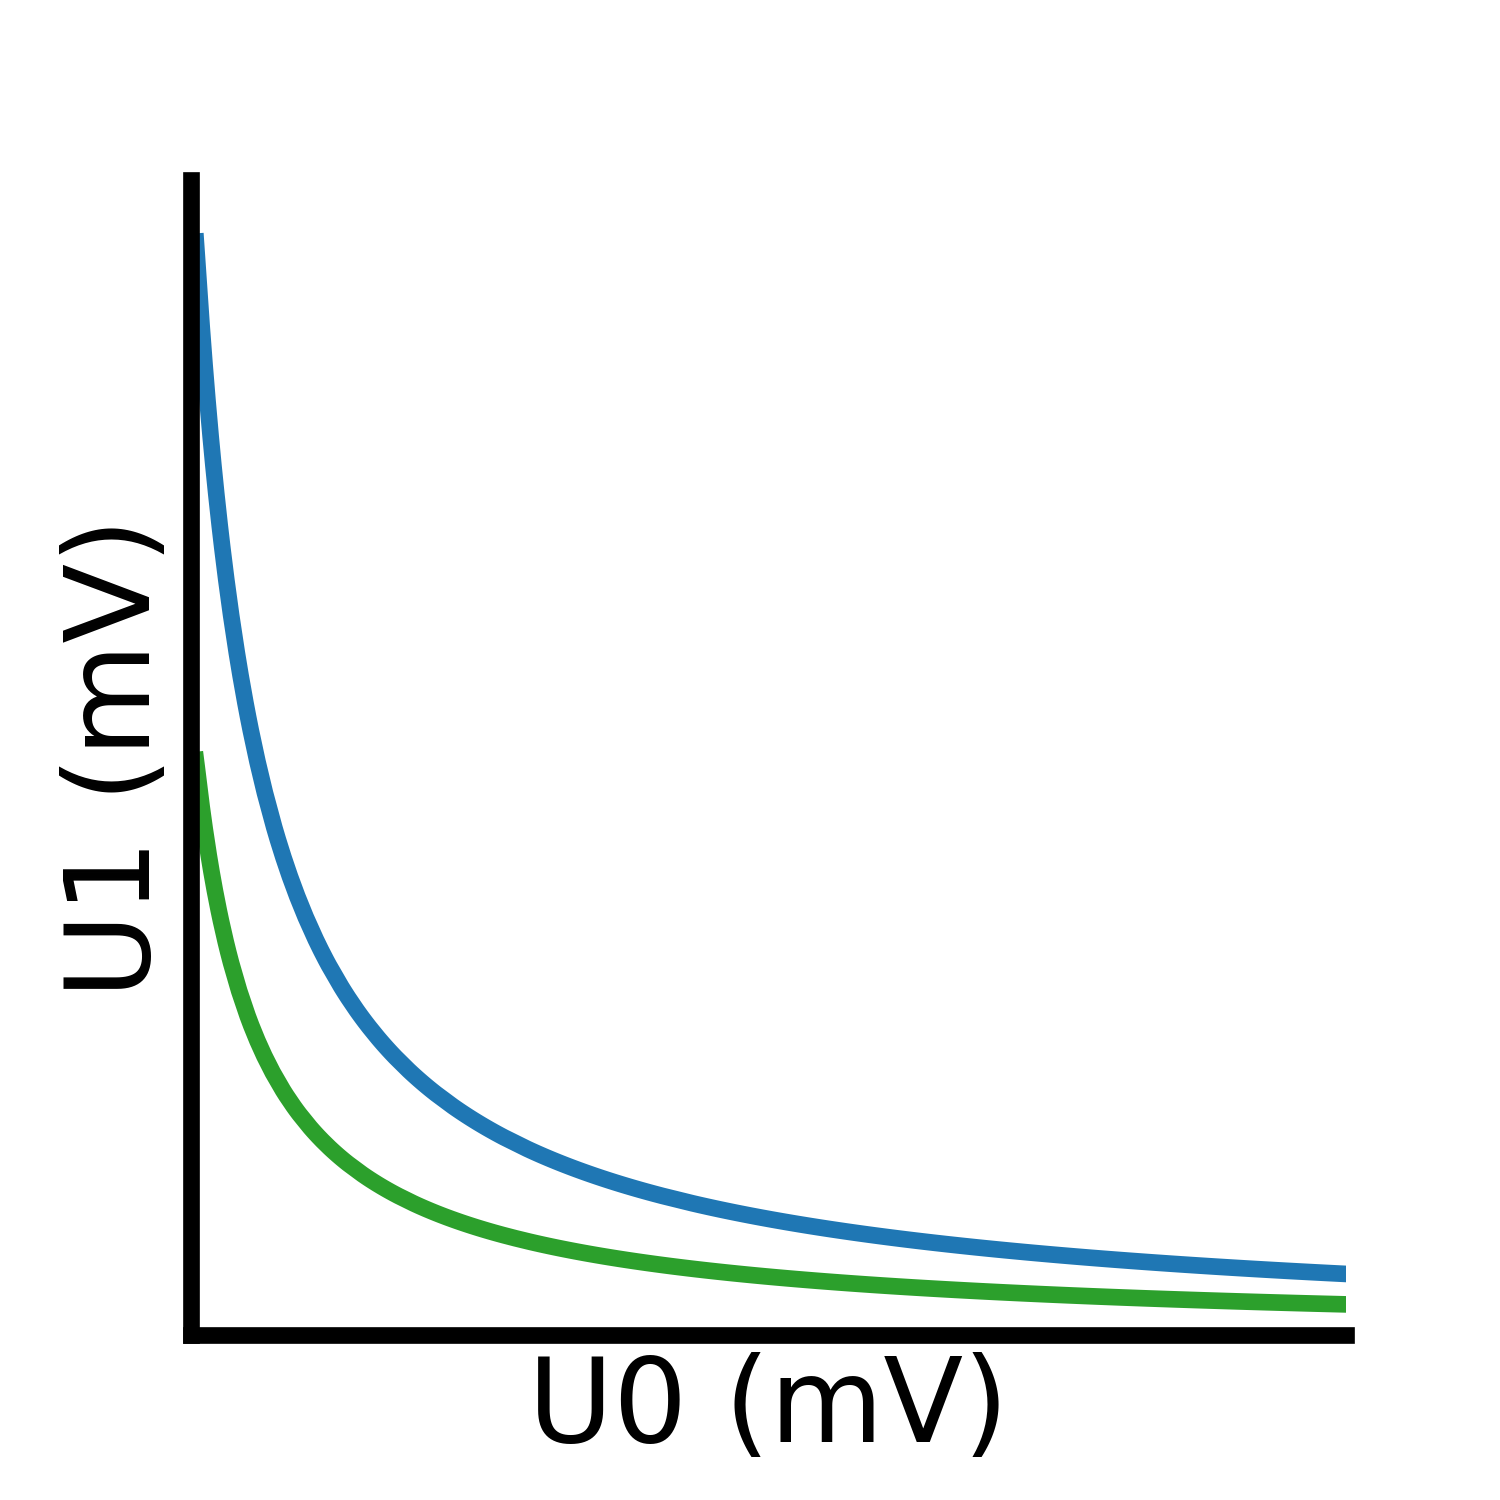
\includegraphics[width=3in]{lit_review/FigDiv} \\
(c) Multiplication & (d) Division \\
\end{tabular}
\caption{Neuron outputs tuned to arithmetic operations}
\label{fig:MathOutputs}
\end{figure}

These subnetworks can be recursively combined to form larger and more intricate
networks that form a controller. This approach allows for the integration of
existing work in controller design with biological inspiration to increase the
effectiveness of the controller when controlling a biologically inspired robot.
This approach also allows for rapid testing and developing new hypotheses about the underlying function of biological systems in a way that typical controller designs do not.


\chapter{Controller Design}
\label{chap:controller_design}
The controller design implemented in code had 3 major goals derived from
requirements and challenges faced with a neural implementation in (cite Hunt's
thesis). See \myref{chap:introduction} for more details.

\begin{enumerate}
\item Increase position accuracy to less than 5 degrees from maximum desired
position
\item Minimize phase shift between desired and achieved trajectory
\item Decrease torque errors between neuron desired model and executed torques
\end{enumerate}

Requirement 2 is fulfilled in
the controller through sensor fusion to estimate state at the time of sensor
readings (assumed to be ``current" time) and then using an internal model of the
joint dynamics to predict the evolution of the joint's position and velocity
given a particular controlling torque. From there, an internal optimization loop
can run to identify a goal torque with sufficient resolution.

An accurate internal model will help meet all 3 requirements. In particular, an
internal model directly solves Requirement 3 by matching controlled torques to
pressures accounting for the pneumatic muscle dynamics. The internal model
designed into the control is designed to adapt to the actual observed
characteristics of the joint, allowing for changing dynamics over time (for
example, adding or removing weight from the robot, degrading pneumatic muscles
or changing positions of other limbs),
adapting to different joints with the same controller and increasing the
robustness of the controller to variations from the original estimated
properties of the robot.

Requirement 1 is met by a combination of the design decisions above and
consistitutes a metric by which to measure the effectiveness of the new design
relative to old designs, regardless of implementation.

\section{Sensor Fusion}

Within the controller, state estimation is done in a relatively simplified
manner. This trades off accuracy for computation time, where the estimation was
refined to run sufficiently accurately that the rest of the system was robust to
small estimation errors.

\subsection{Pneumatic Actuator Simulation/Simplification}

The pneumatic actuators and their existing pressure controller were simulated 
at varying degrees of fidelity ...

% TODO(buckbaskin): finish this thought based on code

\subsection{Centered Divided Difference}

The velocity was estimated with a fixed window of the last 3 position readings.
From there, a centered divided difference formula was used to estimate the
slope and estimate velocity. This was found to be more accurate than a forward
divided difference method only incorporating two points in practice when run
against simulated data.

% TODO(buckbaskin): write the two equations

% TODO(buckbaskin): show a plot with the two different estimations side by side
% to show error

\section{Optimizing Torque Control}

Once the current state of the robot was determined, iteratively optimizing the
desired torque was relatively simple. First, bounds were selected from estimates
of the maximum and minimum (maximum negative) torque that can be applied to the
joint and a forward projection mechanism based on the internal physics model was
used to estimate the resulting position. From there, a binary search procedure
can be used to repeatedly shrink the bounds around the optimal torque. The final
step was to convert the desired torque into a pressure control.

\subsection{Forward Projection of State}

Given the state estimation, project forward.

Also, can use bounds on estimated state, say high and low velocity, to project
forward through multiple iterations, and optimize for the torque that, given the
bounds, is most likely to produce the best result. This work is unnecessary for
a well implemented state estimation system, but is helpful for increasing
robustness to potential sensor reading errors or estimation errors.

% TODO(buckbaskin): complete this thought

\subsection{Torque to Pressure}

% TODO(buckbaskin): complete these two steps
Show the math

Also, talk about designing the desired pressure around the knowledge of a
bang-bang controller under the hood for more accurate pressure control

\section{System Modeling}

Parameter weight updates

\subsection{Actual Error Calculation}

% TODO(buckbaskin): adapt existing work on how the error update should be done
This comes from a writeup that I've already done

\subsection{Evaluation of asymmetric error concerns}o

% TODO(buckbaskin): use some sort of math to show that the over/underestimation
% of damping, etc. can lead to underdamped or overdamped conditions. Prefer
% overdamped control


\chapter{Neuron Design}
\label{chap:neuron_design}
The synthetic nervous system controller is developed with a non-spiking Hodgkin-Huxley neuron model, where the membrane voltage is used as a representation of spiking frequency in a comparable spiking model. The neurons are modeled with a resting potential of -60 mV and a maximum potential of -40 mV for a range of 20 mV.

The voltage for the Hodgkin-Huxley model is determined as follows:

\begin{equation}
C_{m} \dfrac{d V}{d t} = I_{leak} + I_{syn} + I_{app}
\end{equation}

The $I_{app}$ current is arbitrary, and used with multiple neurons in the controller design.
The current terms are defined as follows:

\begin{equation}
I_{leak} = G_{m} * (E_{r} - V)
\end{equation}

\begin{equation}
I_{syn} = \sum_{i=1}^{n} G_{s, i} * (E_{s, i} - V)
\end{equation}

This model does leave out some terms of the Hodgkin-Huxley model. On the other hand, by continuing to follow the work laid out in \cite{NickFunctionalSubnetwork}, the steady state values of a neuron can be arranged in the following equation:

\begin{equation}
U_{post}^{*} = \dfrac{\frac{g_{s}}{R} * U_{pre} * \Delta E_{s}}{1 + \frac{g_{s}}{R} * U_{pre}}
\end{equation}

Through the tuning of the conductivity of the synapse ($g_{s}$), one can engineer the behavior of each type of synapse (see \myref{sec:key_synapses}) to match arithmetic operations. The more complicated operations require the interaction of multiple synapses and neurons, but their behavior is still tuned in the same way.

% TODO(buckbaskin): make the capitalization of the networks consistent

\bbs{Key Neurons and Synapses}
\label{sec:key_synapses}

The neuron controller network is made up of a set of engineered synapses
designed to emulate arithmetic operations. These synapses can be grouped into two
categories: excitatory neurons and inhibitory neurons. 

Most neurons were tuned
via an optimization process to identify the best equilibrium potential and
synaptic conductance based on equations defined in 
\cite{NickFunctionalSubnetwork}. The above equation for determining $U_{post}$ was optimized to match a target dataset that exactly replicated the mathematical operation using a least squares approach.
Some neurons were tuned by hand for specific behaviors in
a subsection of the overall controller.

\bbss{Excitatory Synapses}

Except where otherwise noted, a value of 134 mV was used for the equilibrium
potential of excitatory synapses. The pre-synaptic threshold is -60 mV and the pre-synaptic saturation
level is -40 mV.

\bbsss{Signal Transfer}

The signal transfer synapse is designed to pass the voltage of the input neuron
to the output neuron in the active range of the neuron. The signal transfer synapse is often used to add
the value of two or more neurons together in an output neuron.
The signal transfer synapse has a synaptic 
conductance of 0.115 microsiemens. 

\bbsss{Inverted Signal Transfer}

By combining two signal inversions, a more accurate signal transfer synapse was
created. This involves an extra neuron; however, adding the neuron leads to a more precise
transfer of the voltage level of the input neuron to the output neuron. This tradeoff was used primarily between larger subnetworks. It also helps define boundaries for testing the larger subnetworks. The combined signal transfer synapse was implemented with two Signal Inverter (Stimulated)
synapses.

\bbsss{Signal Amplifier 2x}

The signal amplifier synapse is designed to pass the voltage of the input neuron
to the output neuron with a 2x gain. This synapse was tuned with input values from 0 to
10 mV. Higher inputs saturate the output neuron. It has a synaptic conductance
of 0.23 microsiemens.

\bbsss{Signal Amplifier 4x}

The 4x signal amplifier has the same function as the 2x amplifier but with a larger 
gain. This synapse was tuned with input values from 0 to
5 mV. Higher inputs saturate the output neuron. It has a synaptic conductance
of 0.46 microsiemens.

\bbsss{Signal Reduction 0.2x}

The signal reduction synapse is designed to pass the voltage of the input neuron
to the output neuron in the active range of the output neuron, but with a loss of 0.2x. 
It has a synaptic  conductance of 0.021 microsiemens. The signal reduction synapse was tuned
over the complete range of input values, 0 to 20 mV.

\bbsss{Signal Reduction 0.5x}

The signal reduction synapse has the same function as the 0.2x signal reducer, but with a loss of 0.5x. This signal reduction synapse has a synaptic  conductance of 0.054 microsiemens.

\bbsss{Convert Forward Positive}

The convert forward positive synapse is designed to convert the representation
of a value in a single neuron, for example the neuron that represents the 
position of the joint, to the same value represented in two neurons. This
synapse converts the value when the value is above -50 mV to a positive value between 0 
and 20 mV. The pre-synaptic
threshold of this synapse is -50 mV and its synaptic conductance is 0.115 microsiemens.

\bbsss{Torque Pressure Converter}

The torque pressure converter synapse is designed to perform the torque-pressure
calculation approximation. It has a synaptic 
conductance of 0.048 microsiemens.

\bbss{Inhibitory Synapses}

Except where otherwise noted, the equilibrium potential of inhibitory neurons
is simulated as -100 mV. This is the lowest value possible in the simulation.
The pre-synaptic threshold is -60 mV. The pre-synaptic saturation level is -40
mV.

\bbsss{Signal Inverter}

The signal inverted synapse is designed to decrease the voltage of the output 
neuron proportional to the voltage of the input neuron. It has a synaptic 
conductance of 0.55 microsiemens.

\bbsss{Signal Inverter (Stimulated)}

The signal inverted synapse is designed to decrease the voltage of the output 
neuron proportional to the voltage of the input neuron. This signal inverter (stimulated) synapse is tuned
slightly differently from the standard signal inverter due to an
observed difference in voltage when a stimulus current was applied to the output
neuron along with other incoming synapses. It has a synaptic 
conductance of 0.5 microsiemens.

\bbsss{Signal Inverter Reduction 0.2x}

The signal inverter reduction synapse is designed to decrease the voltage of
the output 
neuron at a 0.2x loss compared to the voltage of the input neuron. This synapse has a 
synaptic conductance of 0.093 microsiemens.

\bbsss{Signal Inverter Reduction 0.5x}

The signal inverter reduction synapse is designed to decrease the voltage of
the output 
neuron at a 0.5x loss compared to the voltage of the input neuron. This synapse has a 
synaptic conductance of 0.22 microsiemens.

\bbsss{Signal Inverter Amplifier 2x}

The signal inverter amplifier synapse is designed to decrease the voltage of
the output 
neuron at a 2x gain to the increasing voltage of the input neuron. It has a synaptic 
conductance of 1.11 microsiemens.

\bbsss{Signal Inverter Amplifier 4x}

The signal inverter amplifier synapse is designed to decrease the voltage of
the output 
neuron at a 4x gain to the increasing voltage of the input neuron. It has a synaptic 
conductance of 2.3 microsiemens.

\bbsss{Integral Inhibitor}

As originally described in \cite{NickFunctionalSubnetwork}, the integral inhibitor synapses are used to mutually inhibit a pair of neurons to hold both 
neurons at a stable value. Without this mutual inhibition, a single neuron acts
as a leaky integrator and its voltage will decay to its resting potential over time without additional input.  The values for this
synapse are based on \cite{NickFunctionalSubnetwork}. The synapse has a  
conductance of 0.5 microsiemens.

\bbsss{Convert Forward Negative}

The convert forward negative synapse is designed to convert the representation
of a value in a single neuron, for example the neuron that represents the 
position of the joint, to the same value represented in two neurons. This
synapse converts the value when the value is below -50 mV to a positive value 
between 0 and 20 mV. The pre-synaptic
saturation of this synapse is -50 mV and its synaptic conductance is 0.5 microsiemens.

\bbsss{Signal Divider}

The signal divider synapse is designed to reduce the effect of another input
synapse, where the reduction increases with increased input voltage to the
signal divider synapse. It is distinguished from the signal multiplier synapse
in that the value never reaches 0. Intuitively, the behavior for large inputs is a replication of 
division where dividing by a large number makes the quantity small but never 0.
It has a synaptic conductance of 20 microsiemens. The equilibrium potential of
the synapse is -60 mV (equal to the resting potential of the input and output
neurons).

\bbsss{Signal Multiplier}

The signal divider synapse is designed to reduce the effect of another input
synapse, where the reduction decreases with increased input voltage to the
signal divider synapse. It is distinguished from the signal divider synapse
behavior in that the value reaches 0. Intuitively, the implementation is a replication of 
multiplication where multiplying by 0 will make any value 0.
It has a synaptic conductance of 19.75 microsiemens. The equilibrium potential 
of the synapse is -61 mV.

\bbs{Sensor Fusion}

The sensor fusion neuron network performs essentially the same function as the
sensor fusion network in the prototype controller. In the synthetic neuron implementation, 3 neurons
represent the 3 sensor inputs available in a joint: position (``Theta"),
extension muscle pressure (``Ext Pres") and flexion muscle pressure
(``Flx Pres"). The outputs for the network are the estimates for current 
position, velocity and acceleration.

\bbss{Velocity Fusion Network Components}

\bbsss{Differentiator Network}

The velocity network is based on the differentiator network presented in 
\cite{NickFunctionalSubnetwork}. The key insight into making a network
of neurons that can estimate the derivative of an input signal is that
the time constants of individual neurons can be independently tuned to 
approximate a single step finite difference method. This itself is based
on a Reichardt detector network as explained in
\cite{NickFunctionalSubnetwork}.

\bbss{Velocity Fusion Network}

The velocity network is based on the Differentiator network. 
The one major change from the network,
as presented, is the inclusion of a second $U_{post}$ neuron to 
represent the negative derivative of the position (negative velocity). See \myref{fig:SensorFusion}.

\begin{figure}
\centering
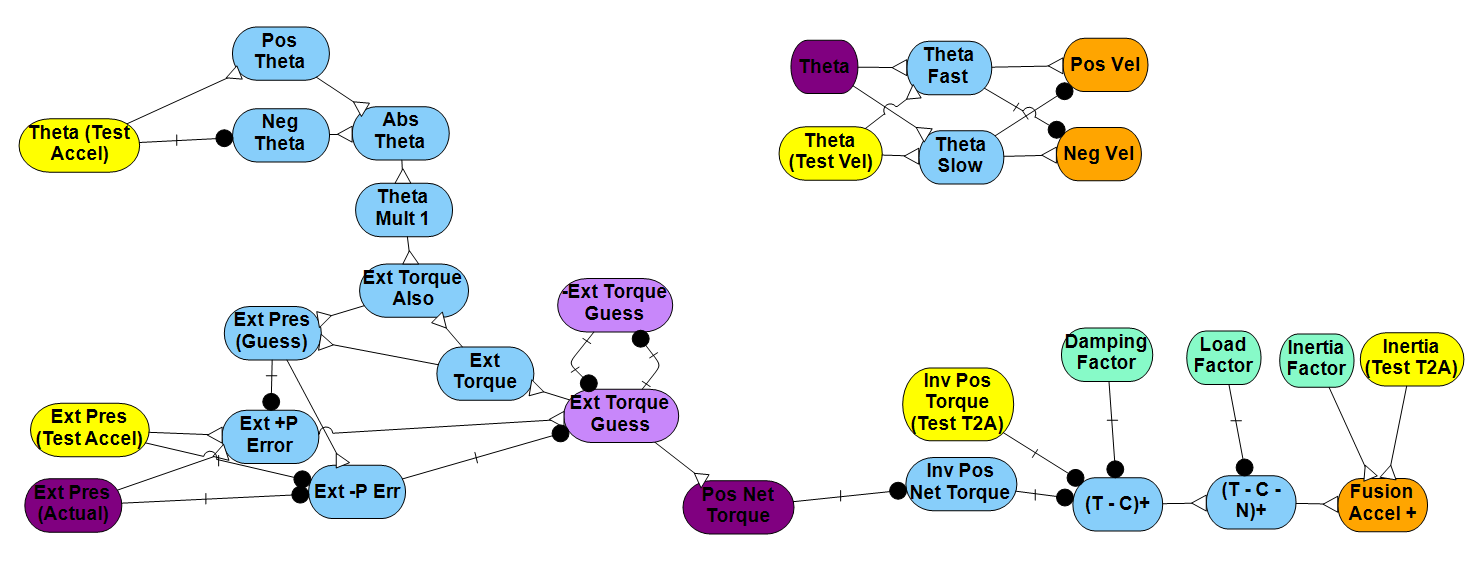
\includegraphics[width=5in]{methods/SensorFusion_Ext}
\caption{Sensor fusion network for acceleration (bottom left) and velocity (top right)}
\label{fig:SensorFusion}
\end{figure}

This represents
a common pattern used across the network where two neurons are used to represent
a single value. One neuron represents positive levels of the variable and is 
at or below resting potential when the value is negative. The other neuron is
above resting potential for negative values and is at or below resting potential
when the value is positive. 

The motivation for increasing the complexity of the
network (often doubling the number of neurons and more than doubling the number of synapses) is to increase the
effective range of values that the neuron can represent at the same fidelity and
to increase the accuracy of zero. When a single neuron represents positive and
negative values of equal magnitude, the value of 0 is represented at 50 mV; 
however, after passing through a signal transfer synapse this value is often
slightly higher, up to 52 mV. This means that comparing the two neurons (the
original neuron and the signal transfer) yields a slightly positive error
instead of near zero error.

\bbss{Acceleration Fusion Network Components}

\bbsss{Absolute Value Network}

Within the acceleration fusion network, the absolute value of the position is
used. This is calculated by first splitting the position into its two neuron
representation. From there, the sum of the two neurons is used as the absolute
value. This takes advantage of the definition of each side of the two neuron
representation falling below resting potential when the other neuron is active.
This means the signal transfer synapse from the below zero neuron will have no
effect.

\bbsss{Integration Network}

The integration network used throughout the neuron controller is based heavily
on the Integrator Network in \cite{NickFunctionalSubnetwork}. Two neurons are
designed to mutually inhibit each other so that the combined pair hold their
values. Individual neurons can be treated as a leaky integrator; however, their
voltage tails off over time if there is no maintenance current. The integration
network itself is tuned by changing the time constant of the component neurons
to adjust how much the voltage of the integrator network changes for an input
current.

\bbsss{Convert Torque to Pressure}

One of the key observations for converting from desired torque to pressure 
within the neuron controller was a pattern observed during simulation. For the
simulated joint, the maximum torque can be applied at an angle of 0 degrees.

\begin{figure}
\centering
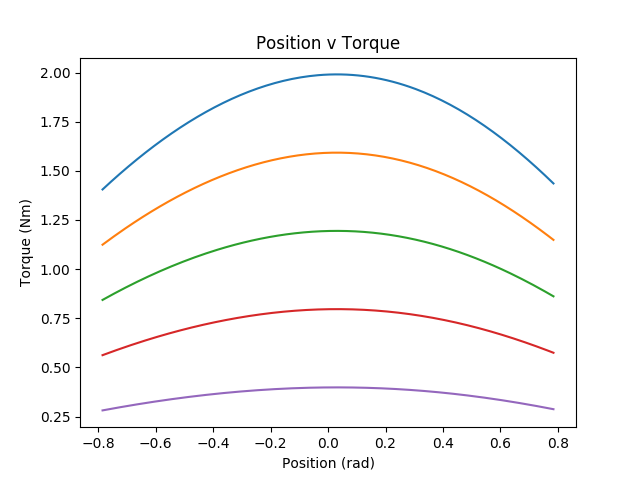
\includegraphics[width=5in]{neuron_design/Pos_v_Torque2.png}
\caption{Position/torque relation for pneumatic muscle actuated joint. See \github{stability/constant\_pressure.py}}
\label{fig:PositionTorque}
\end{figure}

With increasing deflection, there is decreasing torque applied for a given
pressure, or phrased another way, a greater pressure differential is required
for the same desired torque (\myref{fig:PressureTorque} and \github{stability/pressure\_torque.py}). When the calculation is rearranged to calculate
a control pressure from a desired torque at a given position, the relationship
between the two is linear for that position for most desired torques above
0.25 Nm in the simulated joint. Assuming there is some non-zero antagonistic
torque, each actuator should fall into the near-linear range. This allows for
an approximation of the linear section in the neuron model.

\begin{figure}
\centering
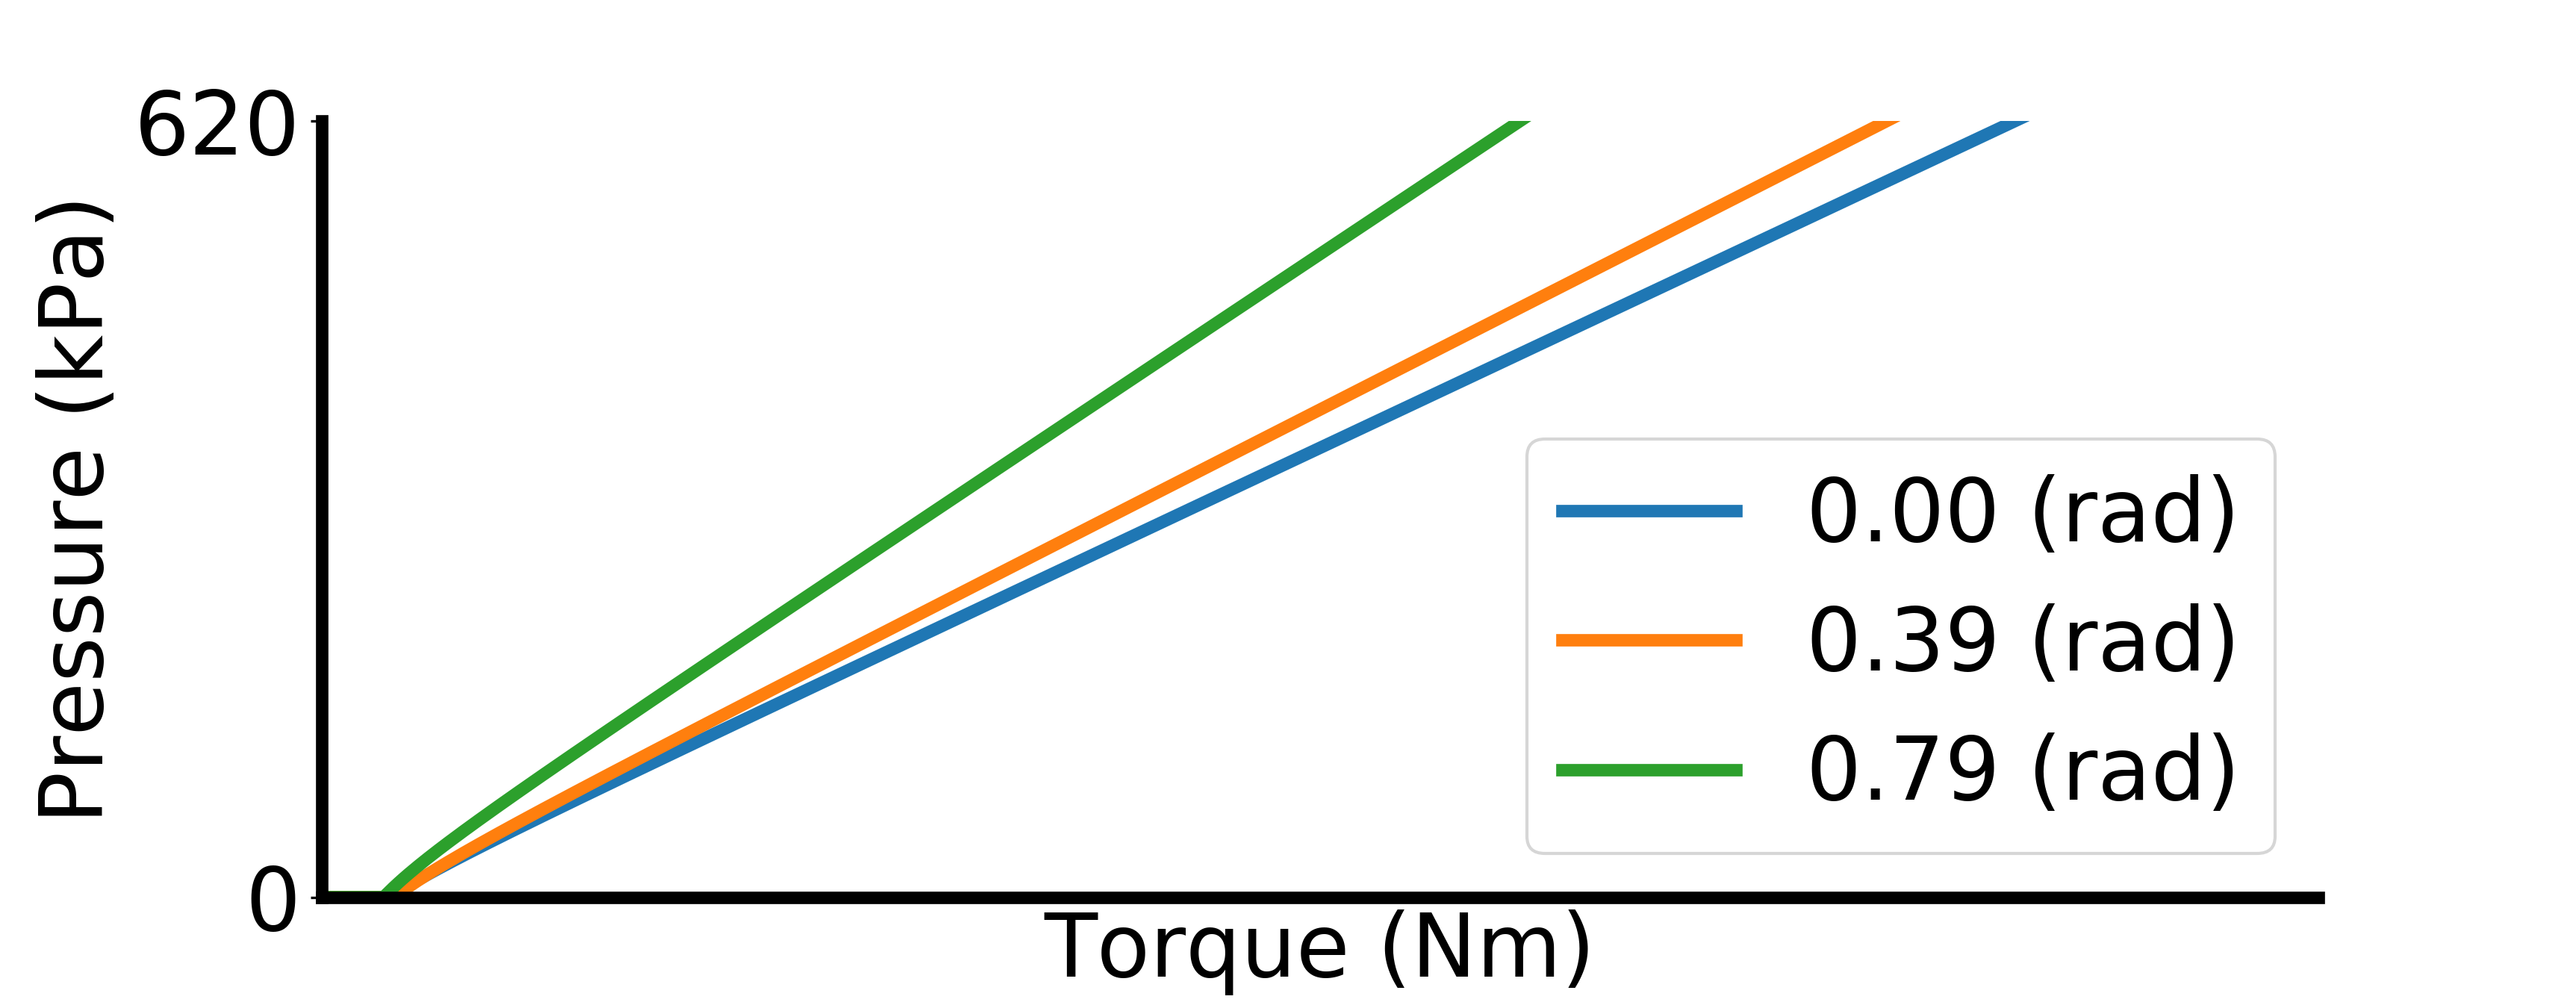
\includegraphics[width=5in]{neuron_design/FigPressureTorque}
\caption{Torque/Pressure relation observed in simulation}
\label{fig:PressureTorque}
\end{figure}

The neurons approximate the torque/pressure relationship using a multiplication synapse added
to a signal transfer synapse. The multiplication takes the scaled absolute 
value of the position as input, so that as the position of the joint reaches
the joint limit, the slope of the torque to pressure curve increases. This
approximates the observations in simulation with a relatively simple neuron
network. See \myref{fig:T2PNetwork} for the assembled network.

\begin{figure}
\centering
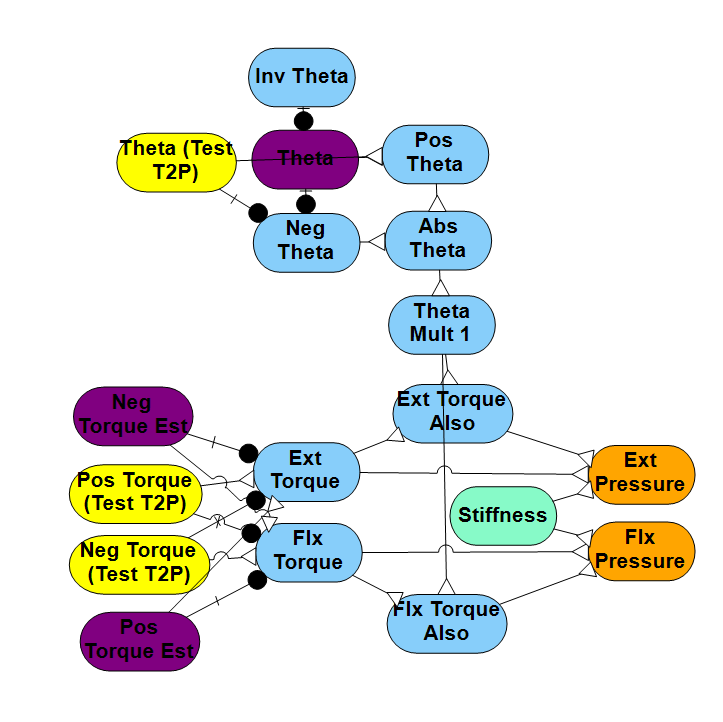
\includegraphics[width=5in]{methods/TestVisualT2P}
\caption{Torque to pressure conversion network}
\label{fig:T2PNetwork}
\end{figure}

\bbsss{Pressure Estimation Loop}

Within the Acceleration Network, there is a feedback loop that is used to 
estimate the torque applied by a given pressure. First, the loop ``initializes"
with an extension torque guess from the integrator. Second, the extension
torque is converted into extension pressure. Third, the estimated extension
pressure is compared with the sensed pressure. If there is an delta between the
two, the extension torque guess is modified in turn and the cycle repeats.

This architecture is mirrored for flexion torque.

\bbsss{Torque to Acceleration Network}

The torque to acceleration network is built up in 3 stages. First, a damping 
term is subtracted or added based on the current velocity and the estimated
damping factor. Second, the conservative load is applied to the joint. Third,
the acceleration is attenuated proportional to the mass with a signal divider
synapse.

The scaling of the damping factor is the most complicated component of this
network. First, the estimated damping factor is scaled based on the velocity 
with a multiplication synapse to ensure that damping has no effect on acceleration
when the velocity is zero. Second, the damping factor is then applied with both positive and
negative velocities (in a split representation) to the positive and negative
acceleration terms. Due to the design choice of representing the velocity as two
neurons, one term will be 0 and the other will either have a 
non-zero effect. In code, the comparable calculation would be done as an if statement. In neurons,
all the values and effects are calculated in practice, but only some are passed
through the network.

\bbss{Acceleration Fusion Network}

The acceleration fusion network is a combination of an integrator, absolute
value network, the pressure estimation loop and a torque to acceleration
network. In total, the network uses a combination of smaller networks to
estimate the torque applied from sensed pressure and then combine the extension
and flexion torques together to get a net torque and acceleration. For the complete network, see \myref{fig:SensorFusion}.

\bbs{Optimizing Torque Control}

The torque control network uses a feedback loop to optimize the
control torque. The network takes the estimated position and velocity from the 
sensor fusion network and the desired position from a trajectory generator
network (ex. a CPG) and outputs the torque to best follow that trajectory.
See \myref{fig:TorqueOptimizationNetwork} for the complete network.

\begin{figure}
\centering
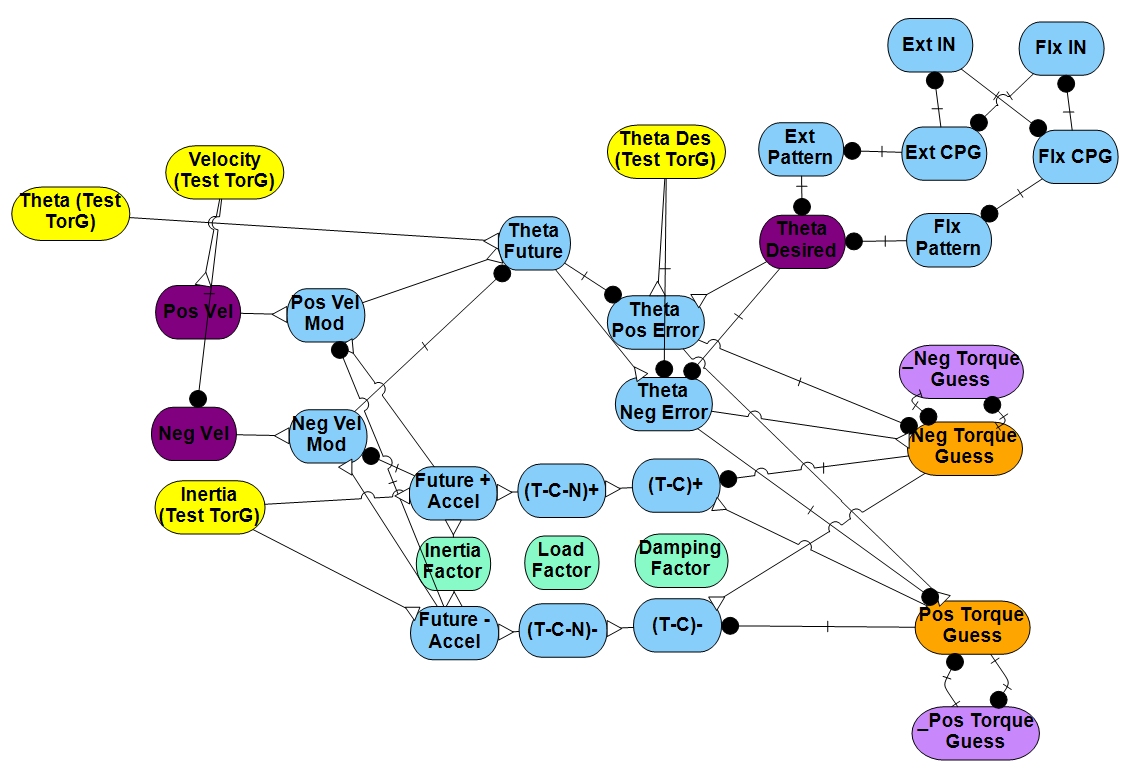
\includegraphics[width=5in]{methods/TorqueOptimization}
\caption{Feedback loop for determining the desired control torque}
\label{fig:TorqueOptimizationNetwork}
\end{figure}

\bbss{Optimizing Torque Control Components}

\bbsss{Torque Estimation}

The first step in the torque control network is a torque estimate. This is built
as an integration network.

\bbsss{Torque to Acceleration}

This torque to acceleration network is calculated in the same manner as above.
The principle difference is that the source of torque is an desired control
torque instead of the estimated applied torque of the actuators.

\bbsss{Velocity Modification}

The velocity modification network takes the current velocity in and adjusts for
the acceleration. Based on the estimated update rate of the controller, the
change in velocity is linear in acceleration.

\begin{equation}
\dot{\theta}_{future} = \dot{\theta}_{current} + \ddot{\theta} * \delta t
\end{equation}

This is encoded as a constant gain (calculated to be 0.2x) to be incorporated 
into to the velocity voltages.

\bbsss{Position Modification}

The position modification network takes the modified velocity in and adjusts the
future position for a time step in the same method as the velocity modification
network.

\begin{equation}
\theta_{future} = \theta_{current} + \dot{\theta}_{future} * \delta t
\end{equation}


\bbsss{Position Comparator}

The position comparator estimates the error between where the joint will be at
the future point and time and where the trajectory generator wants the joint
to be. This error is used as feedback to directly modify the torque estimate.
This network geometry allows for easy incorporation of other metrics as well.
For example, if the position estimation is noisy, multiple forward projections
can be made for upper and lower bounds and the torque can be optimized to 
minimize an error function over all projected locations.

\bbss{Torque Control Network}

The overall feedback loop and torque control network is a combination of pieces
that joint together to approximate
Newton's Method for finding the root of the error function.

The original 
controller used a bounded bisection method that proved less suited for 
implementation in neurons. The bisection method was originally chosen because
it would always converge or have a well defined behavior when the desired
position fell outside the bounds.

\begin{equation}
\theta_{future} = \theta_{current} + (\dot{\theta}_{current} + \ddot{\theta} * \delta t) * \delta t
\end{equation}

\begin{equation}
\theta_{future} = \theta_{current} + \dot{\theta}_{current} * \delta t + \ddot{\theta} * \delta t^{2}
\end{equation}

\begin{equation}
\dfrac{\partial \theta_{future}}{\partial \ddot{\theta}} = \delta t^{2}
\end{equation}

The derivative of the position is constant with respect to the controlled value
$\ddot{\theta}$. Therefore, Newton's Method should also always converge and it is a suitable replacement for the bisection method in the synthetic neuron
controller. In practice, Newton's Method should work well with many error functions; however,
a more complicated error function involving multiple independent error 
components may exhibit local minima and a more complex root finding feedback
method may be required.

\bbs{Torque to Pressure}

The torque to pressure section of the network is smaller than the rest of the 
major components. It is built in the same way as the torque to pressure inside
the sensor fusion pressure to torque network. In the sensor fusion application,
the network is used in a forward capacity inside of a feedback loop that ends
up performing an inverse. This network is much more simple because the network
is used only in a forward capacity to compute the desired pressures.

One additional modification to the network is the inclusion of a stiffness
parameter neuron. This controls any desired overlap in the antagonistic control
to increase or decrease joint stiffness manually.

\bbs{System Modeling}

The system modeling network compares the predicted location of the joint from 
the last control iteration with the current position. Using the error 
calculations discussed in \myref{chap:controller_design}, the neuron network
can calculate the weight updates for its internal estimate of damping and 
conservative load. The equations are as follows:

\begin{equation}
\lambda 
=
- \dfrac{2M}{\delta t^{2}} \dfrac{\theta_{err}}{1 + \dot{\theta}_{0}^{2}}
\end{equation}

\begin{equation}
C_{err} = \lambda \dot{\theta}, N_{err} = \lambda
\end{equation}

\begin{figure}
\centering
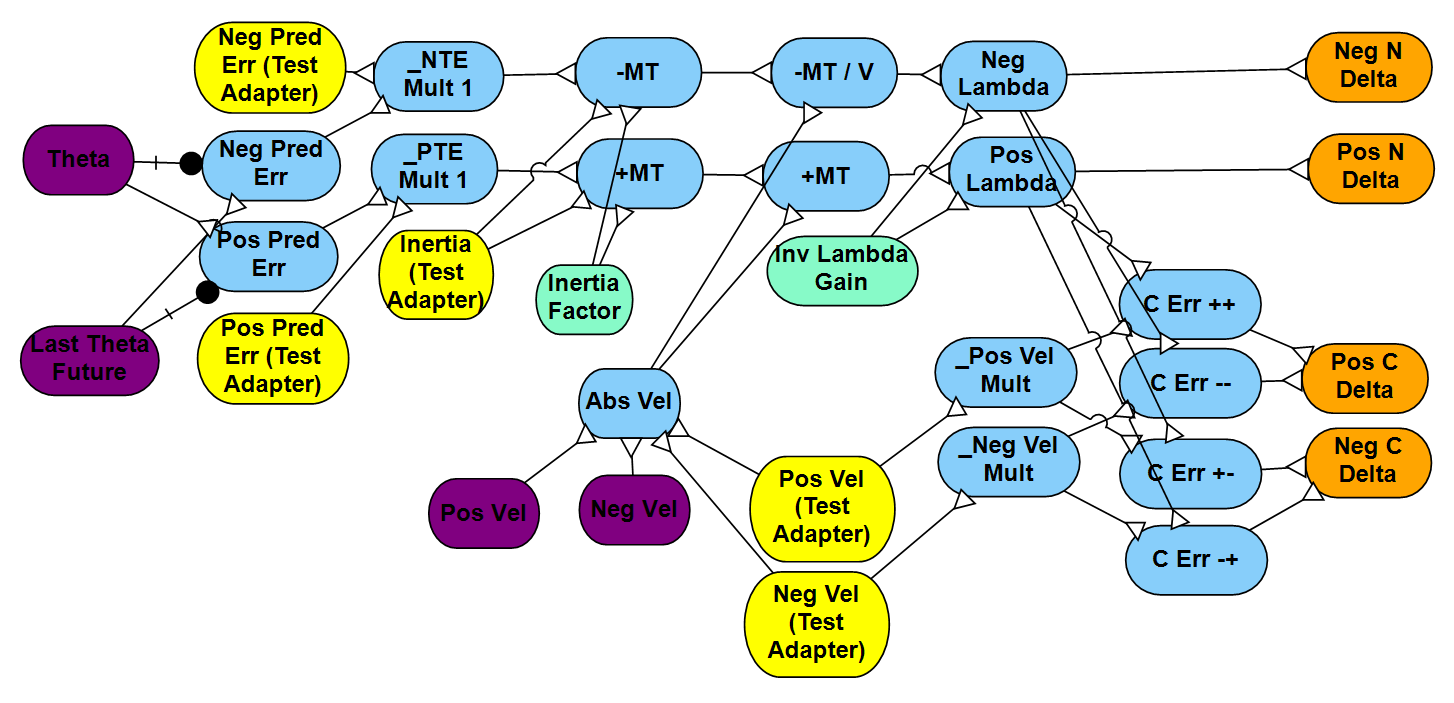
\includegraphics[width=6.5in]{methods/SystemModel_Test}
\caption{System modeling network}
\label{fig:SystemModelNetwork}
\end{figure}

\myref{fig:SystemModelNetwork} shows the complete network.

\bbss{System Modeling Components}

\bbsss{Theta Delay}

The most unique component of the system is the delayed neuron that approximates
the estimated position of the joint. This is done with a signal transfer
synapse and a single neuron with a time constant that is tuned to the controller
update rate.

\bbsss{Prediction Error}

The prediction error is calculated in both a dual neuron representation. The
error is then multiplied with the inertia, again resulting in a dual 
representation of the positive and negative quantity. This matches the behavior
expressed in the first term of the update equation to calculate $\lambda$.

\bbsss{Velocity Correction}

The absolute value of the velocity is used along with a signal divider. This
matches the second term of the equation to calculate $\lambda$. In practice,
the divider network is one of the networks that fits closely to a term like
$\dfrac{1}{1 + x^{2}}$. One potential improvement to the network is to fit
a custom synapse or subnetwork to better fit the term; however, the velocity estimate is not
currently a major source of error.

\bbsss{Lambda Calculation}

The calculation of $\lambda$ is completed with the addition of a gain term. This
allows for the scaling of the updates and behaves in a similar way to the 
learning rate in a neural network. A single data point may be noisy, but if a 
series of updates suggest the same parameter update, the network will adjust the
parameter.

\bbsss{Calculating $\Delta N$}

The calculation for the conservative load is simply a signal transfer from the scaled lambda, following the given equation.

\bbsss{Calculating $\Delta C$}

The calculation for the damping factor update is more involved. In particular,
the complexity comes from the fact that the sign of the update changes with the
sign of the velocity and the positional error. Intuitively, the change in sign occurs when
damping opposes velocity, but conservative loads (as modelled) don't depend on
velocity. For example, a positive velocity and positive $\lambda$ means that 
less actual damping occurred than was expected, but a negative velocity with a 
positive $\lambda$ means that more damping occurred than was expected.

To perform the damping factor calculation in neurons, the velocity and $\lambda$ are 
calculated for all sign pairs. From there, the correct outputs are connected.
Following the example above, a positive velocity and positive $\lambda$ transfer
their signal to the positive C delta, which then connects to the damping factor 
to drive the stored value down. For a positive lambda and a negative velocity, the ``C Err -+" neuron activates and transfers activation to the negative C Delta output.

This implementation relies on the dual neuron representation for values to drive
the correct output. Either the positive or negative neuron will be active in the
velocity and $\lambda$ values, therefore only one of the 4 combination neurons
will be active meaning that only the correct sign of the output value will be
active, maintaining the correctness of the dual neuron representation in the 
output. This implementation replaces a series of if statements that may appear
in a code-defined controller and shows an additional advantage of using two
neurons to represent a value in a functional subnetwork. When connected 
correctly, the dual neuron representation of single values allows for easier sign flipping, easier validation of correctness
by checking edge connectivity, and easier testing.

\bbs{Combined Controller Network}

The fully combined network implements
a controller by combining the 4 large subnetworks. First, sensor data is passed
through a sensor fusion network. The state estimation output of the sensor 
fusion network are then passed into the torque optimization network. The 
selected torque is then passed through one more subnetwork to convert the
desired torque into pressures for the actuators.

This leaves the system model subnetwork. This last subnetwork is connected to 
the state estimation values and the internal projection and observes the 
differences between the forward prediction and reality. This observer then 
updates key model parameters to improve the controller over time while 
maintaining a controller that avoids excessive oscillation. 


\chapter{Testing/Methods}
\label{chap:methods}
\section{Simulation}

\subsection{Animatlab}

Animatlab is a simulation environment that combines a physics engine with a
neuron simulation tool. It is very helpful for integrating physical systems
and sensor information easily into a synthetic nervous system.

The design tools for defining and testing a nervous system were also instrumental
to the success of the new controller design.

\subsection{Python Numerical Simulation}

During the development of the original controller design, an additional
simulation environment was created in Python. Due to the complicated nature of
the controller design, it was impractical to prove the stability and other
properties of the controller directly, especially with changing internal
parameters. Instead, the Python simulation environment was used to gradually add
in expected physical effects to see how the algorithm behaved.

The pneumatic actuators and their existing pressure controller were simulated 
at varying degrees of fidelity. Originally, a simple model of the actuators
was used that emulated their non-linear behavior for applying torque, but didn't
include damping effects, load or limitations of the underlying pressure
controller. Over time these effects were added in until a high fidelity model of
a joint was controlled with the algorithm. This simulation environment also
enabled the testing and verification of a simplified internal model for
replication within the neuron controller. Without the Python simulation
environment, this evidence-based design of models would not have been as easy to
iterate.

\section{Testing and Verification}

One of the key steps for verifying the neuron controller was a series of tests
using the DataTool functionality of Animatlab. By simulating inputs to subsets
of the network, the output can be verified against the Python controller
implementation or other pre-computed values. This independent testing further
reinforces the value of the functional sub-network approach.

\subsection{Neurons}

One of the most important aspects of the functional subnetwork approach is that
individual subnetworks can be tuned, verified and then combined with the larger
network. In order to better tune individual networks, a testing rig was set up
within the larger network to allow for subnetwork verification. The typical
interface neurons are disabled and special test driver neurons (highlighted in
yellow) are enabled. This allows for the driving of custom input signals and
combinations of signals in order to verify the output value and speed. 
See \myref{fig:TestNetworkT2P} for a good example.

\begin{figure}
\centering
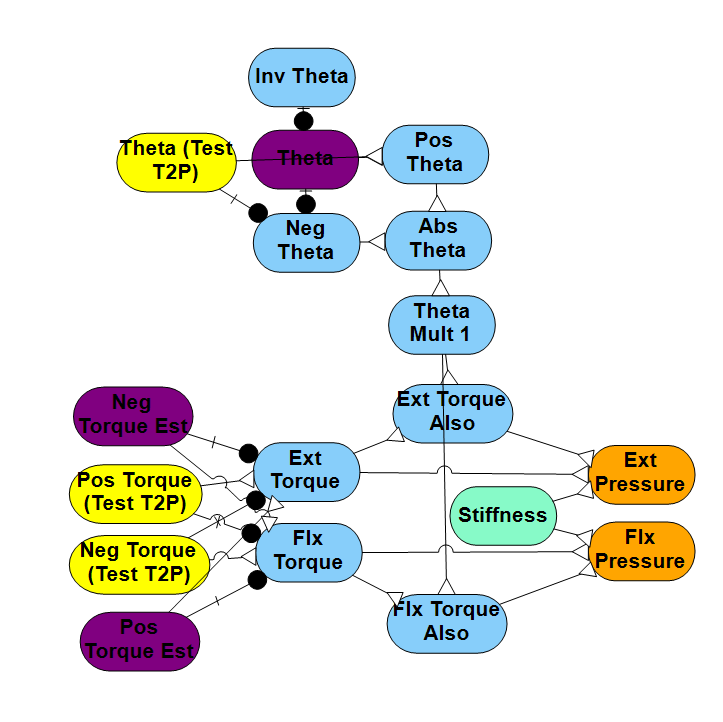
\includegraphics[height=3.5in]{methods/TestVisualT2P}
\caption{Torque to Pressure network with test and actual inputs shown}
\label{fig:TestNetworkT2P}
\end{figure}

This particular network is designed to convert a desired torque from the rest
of the network to the pressure for the extension and flexion pneumatic actuators.
With this network, the input neurons (in purple)
are disabled for testing and the test neurons are enabled. From there, inputs
are driven, as seen in \myref{fig:TestNetworkInputs}. This allows the inputs to 
be mapped to real world values, the real world inputs to be mapped to outputs, 
and the real world outputs to be mapped back to neuron voltages. Through this
a test framework is built where the output can be visually compared to the 
reference to ensure neuron networks are working as intended. See 
\myref{chap:results} for the results of the tests that were run.

\begin{figure}
\centering
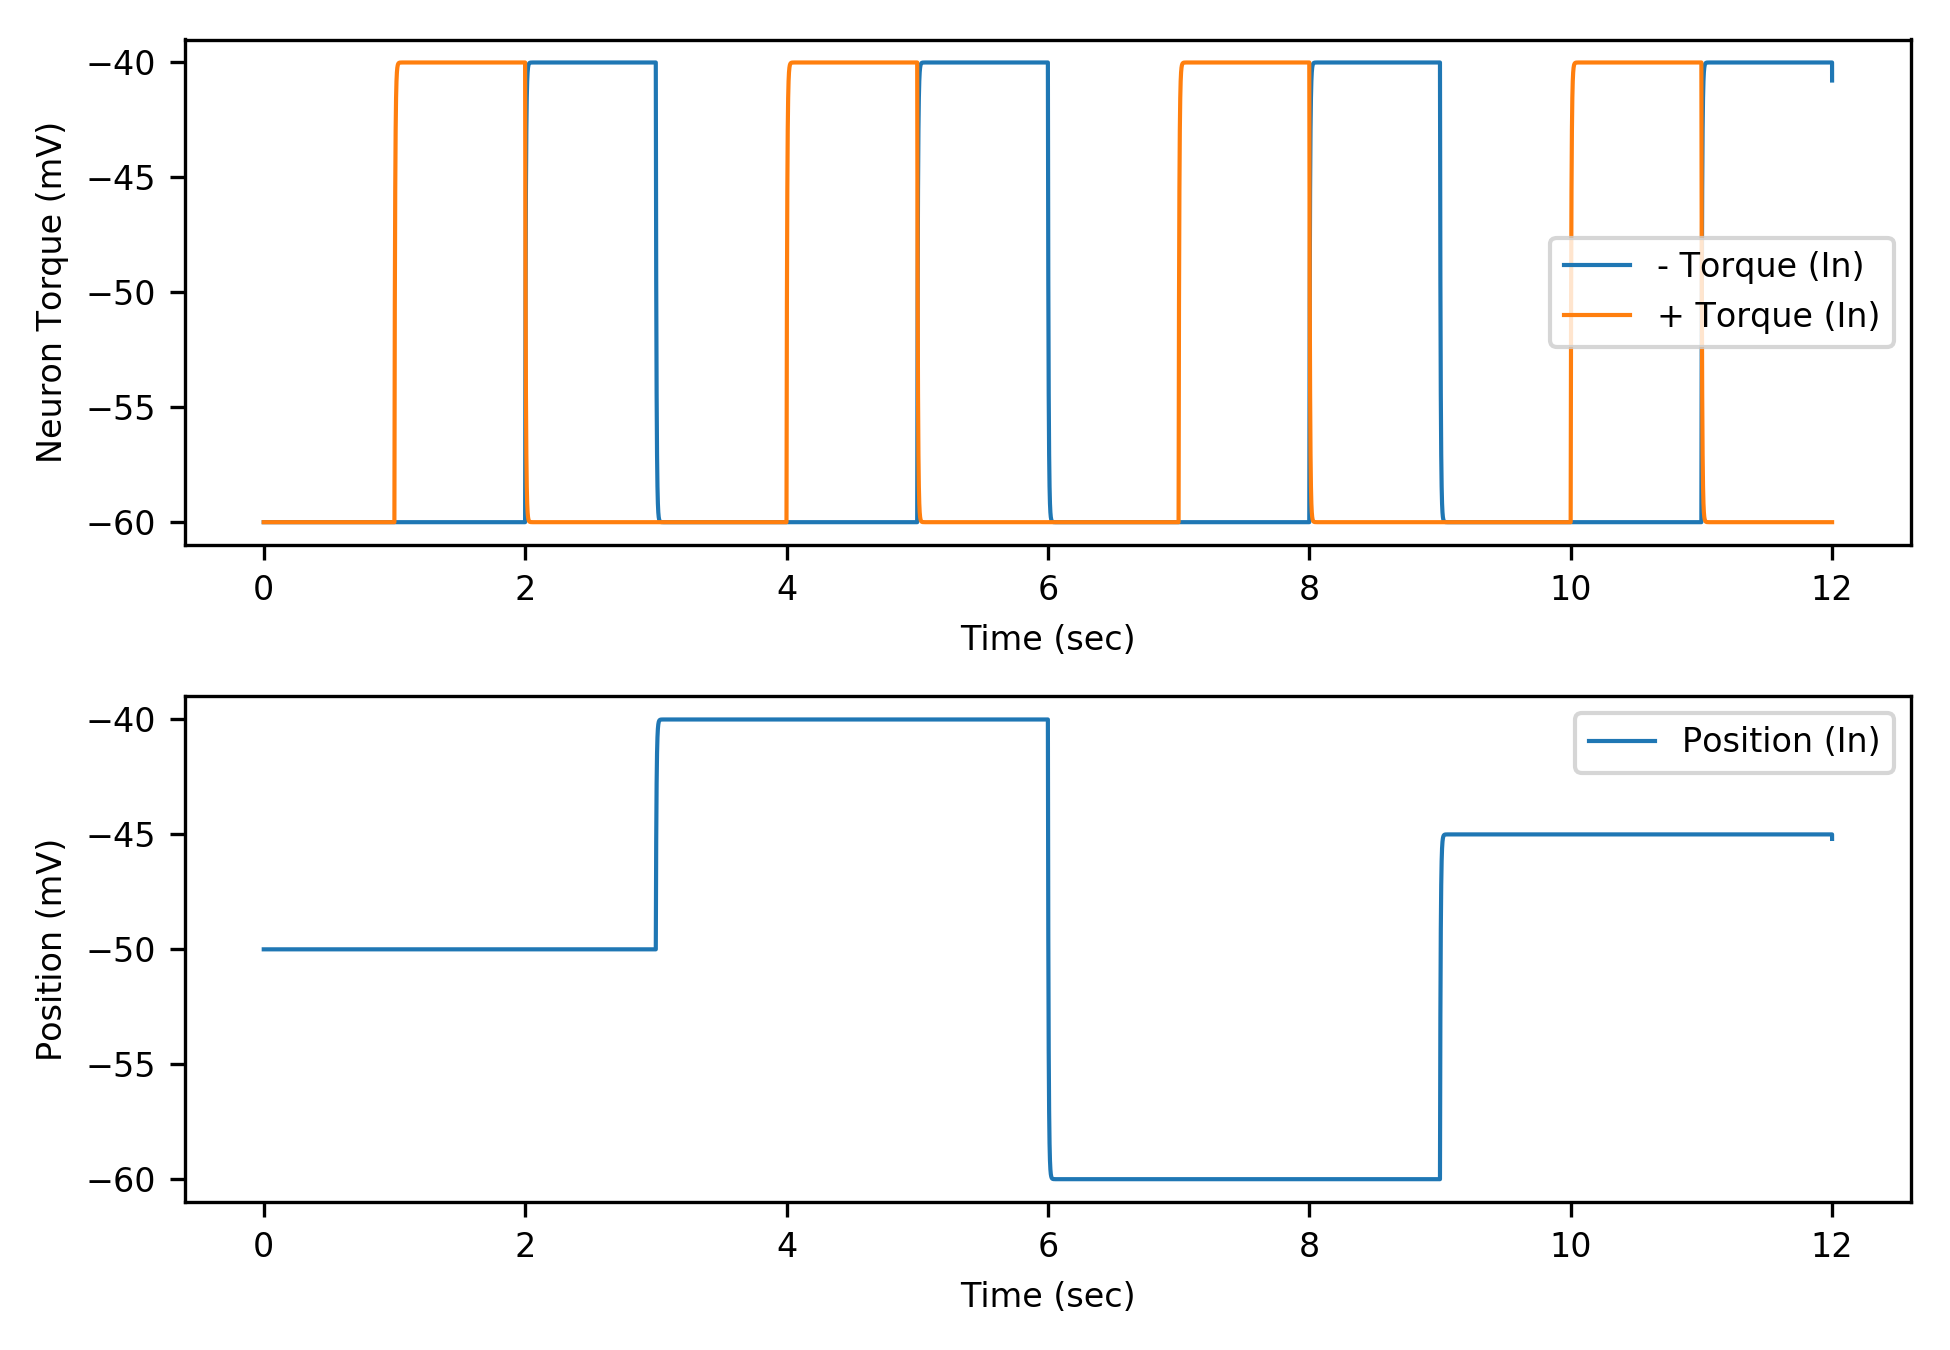
\includegraphics[height=3.5in]{methods/T2PInput}
\caption{Drive inputs to test the pressure network}
\label{fig:TestNetworkInputs}
\end{figure}

The test frameworks can be rigged at multiple levels to enable testing of
individual units and the integration of units in the style of unit tests and
integration tests from a more traditional software background.


\chapter{Results}
\label{chap:results}
\bbs{Simulation}

Antagonistic actuators were simulated at various pressures to better understand
their behavior using \github{stability/constant\_pressure.py}. In \myref{fig:AntagonisticPressureTorque}, the extension
actuator was set to a constant 500 kPa. The pressure in the flexion actuator was
varied, and the torque was plotted for a range of actuator angles. This model of
torque generated was used in ongoing work to help better understand joint
dynamics and improve the performance of the controllers.

\begin{figure}
\centering
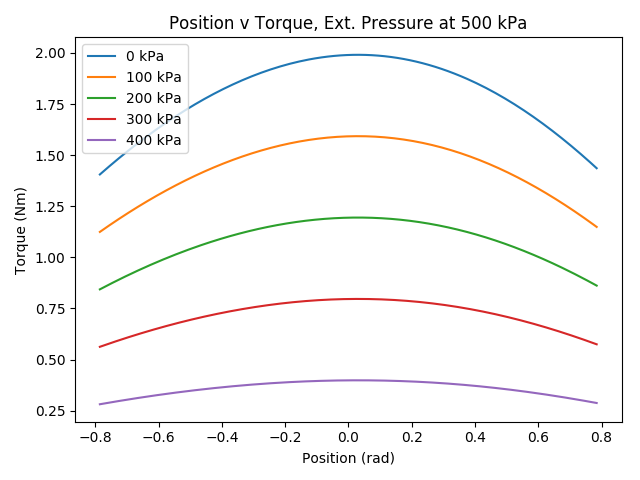
\includegraphics[height=3.5in]{results/Pos_v_AntagTorque}
\caption{Relation between joint position, actuator pressures and
torque applied. Extension actuator pressure was set to 500 kPa and flexion was
set as indicated.}
\label{fig:AntagonisticPressureTorque}
\end{figure}

During the characterization of the joint, simulations were run to determine the
dominant effects between inertia, damping and static loads using \github{stability/max\_torque.py}. The relative 
magnitudes of the acceleration, velocity and position are shown in 
\myref{fig:MaxTorque}, along with the
torque. For the simulated joint, the dominant effect was the inertia; however,
for a robot carrying varying loads, the inertia will not always be the dominant factor. The 
maximum torque required to execute the known trajectory is also later used as a
metric for measuring the efficiency of the controller. A controller that is too
aggressive for the trajectory (ex. too high gains on a proportional controller)
will request larger than needed torques during trajectory execution. An ideal
controller will always follow the trajectory with the exact torque needed during steady state operation.

\begin{figure}
\centering
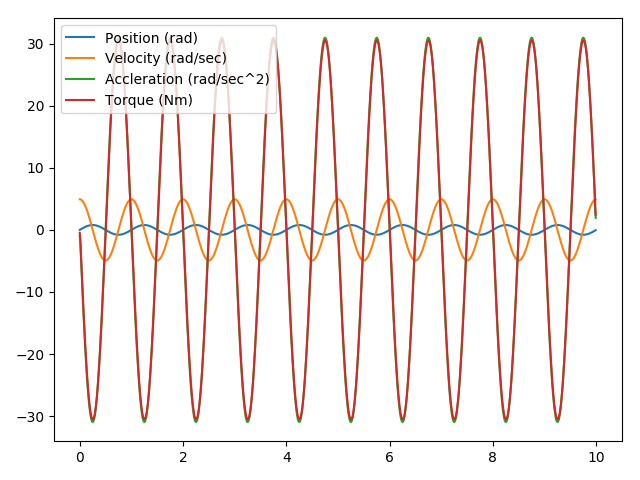
\includegraphics[height=3.5in]{results/Max_Torque}
\caption{Comparing the effects of inertia, damping and static loads. Torque follows acceleration, which suggests that inertia dominates for this simulation}
\label{fig:MaxTorque}
\end{figure}

\bbs{Python Controller}

The prototype controller written in Python was used to demonstrate the stability
and tracking capabilities of the general algorithm. The prototype controller also was used to find a
suitable simplification of the internal model that was sufficiently accurate for
optimization but had minimal parameters to tune.

\bbss{Simplified Controller}

The simplified controller demonstrated effective control once the weight updates
were combined with a suitable starting state. \myref{fig:SimplifiedTracking}
demonstrates the progression from original state to a stable and accurate
control of joint position. The blue line is the desired trajectory, with purple
used to highlight error bounds of $\pm$ 1 degree. Orange indicates the actual
position of the joint, and the green line indicates the internal state
estimation.

\begin{figure}
\centering
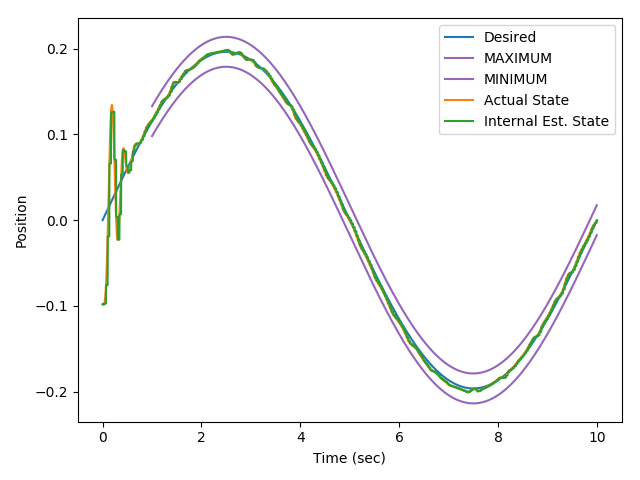
\includegraphics[height=4in]{results/State_Estimation}
\caption{Tracking improves with improved state estimation and internal model
updates}
\label{fig:SimplifiedTracking}
\end{figure}

\bbss{Static Controller}

During testing, the need for an internal model update was verified through 
tests where the optimization loop was applied with variations on 
parameters using \github{stability/simple\_mass\_model.py}. One example was varying mass. For correct values, such as 
\myref{fig:StateEstimationPerfect}, the system worked within tolerances. When 
mass was underestimated (see \myref{fig:StateEstimationLowMass}), the tracking 
performance degrades to smoothly fail required tracking accuracy. On the other 
hand, over-estimating the inertia caused aggressive oscillation and underdamping (see \myref{fig:StateEstimationHighMass}). Based on these tests, the assumption 
that the internal model needs to update was validated.

\begin{figure}
\centering
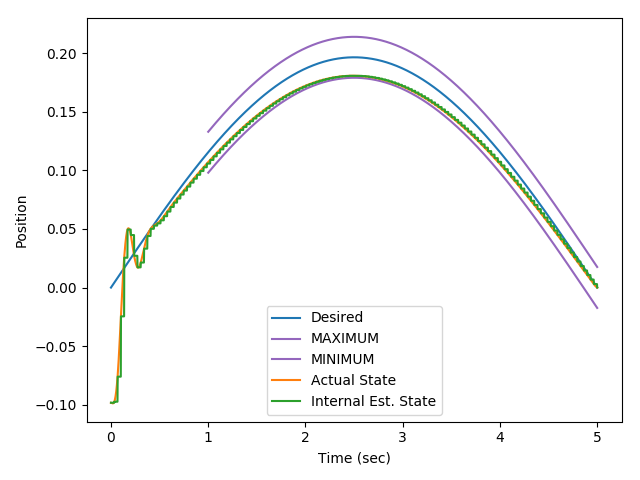
\includegraphics[height=4in]{results/State_Estimation_Perfect}
\caption{Accurate tracking with a good internal estimation of mass}
\label{fig:StateEstimationPerfect}
\end{figure}

\begin{figure}
\centering
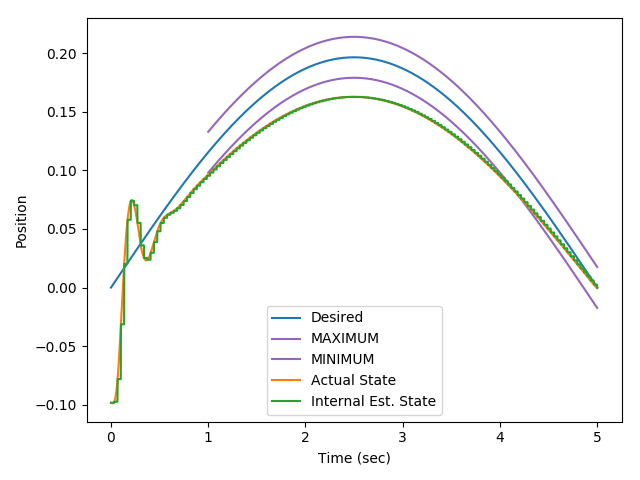
\includegraphics[height=4in]{results/State_Estimation_LowMass}
\caption{Overdamped tracking with an internal underestimation of mass}
\label{fig:StateEstimationLowMass}
\end{figure}

\begin{figure}
\centering
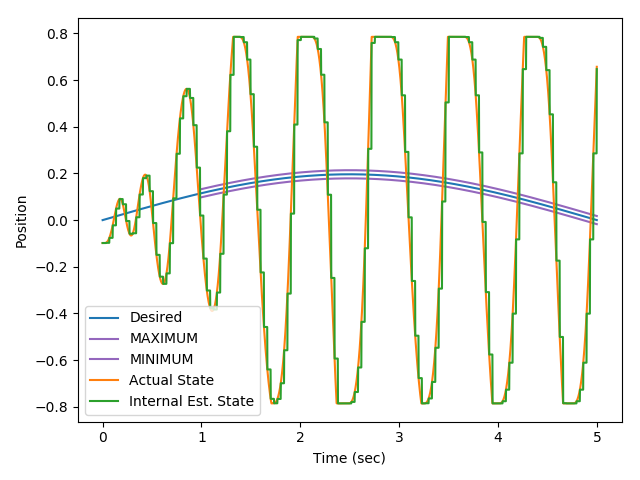
\includegraphics[height=4in]{results/State_Estimation_HighMass}
\caption{Underdamped failure with an internal overestimation of mass}
\label{fig:StateEstimationHighMass}
\end{figure}

\bbss{Simple Parameter Estimation}

The original model for parameter updates was to calculate the sign of the update
and make a uniform incremental change in that direction. In practice, the constant uniform update
resulted in near-perfect tracking; however, the weight updates themselves were continually varying instead of stabilizing to a true value. See \myref{fig:StateUpdateSimple} and \github{stability/simple\_mass\_model.py}.

\begin{figure}
\centering
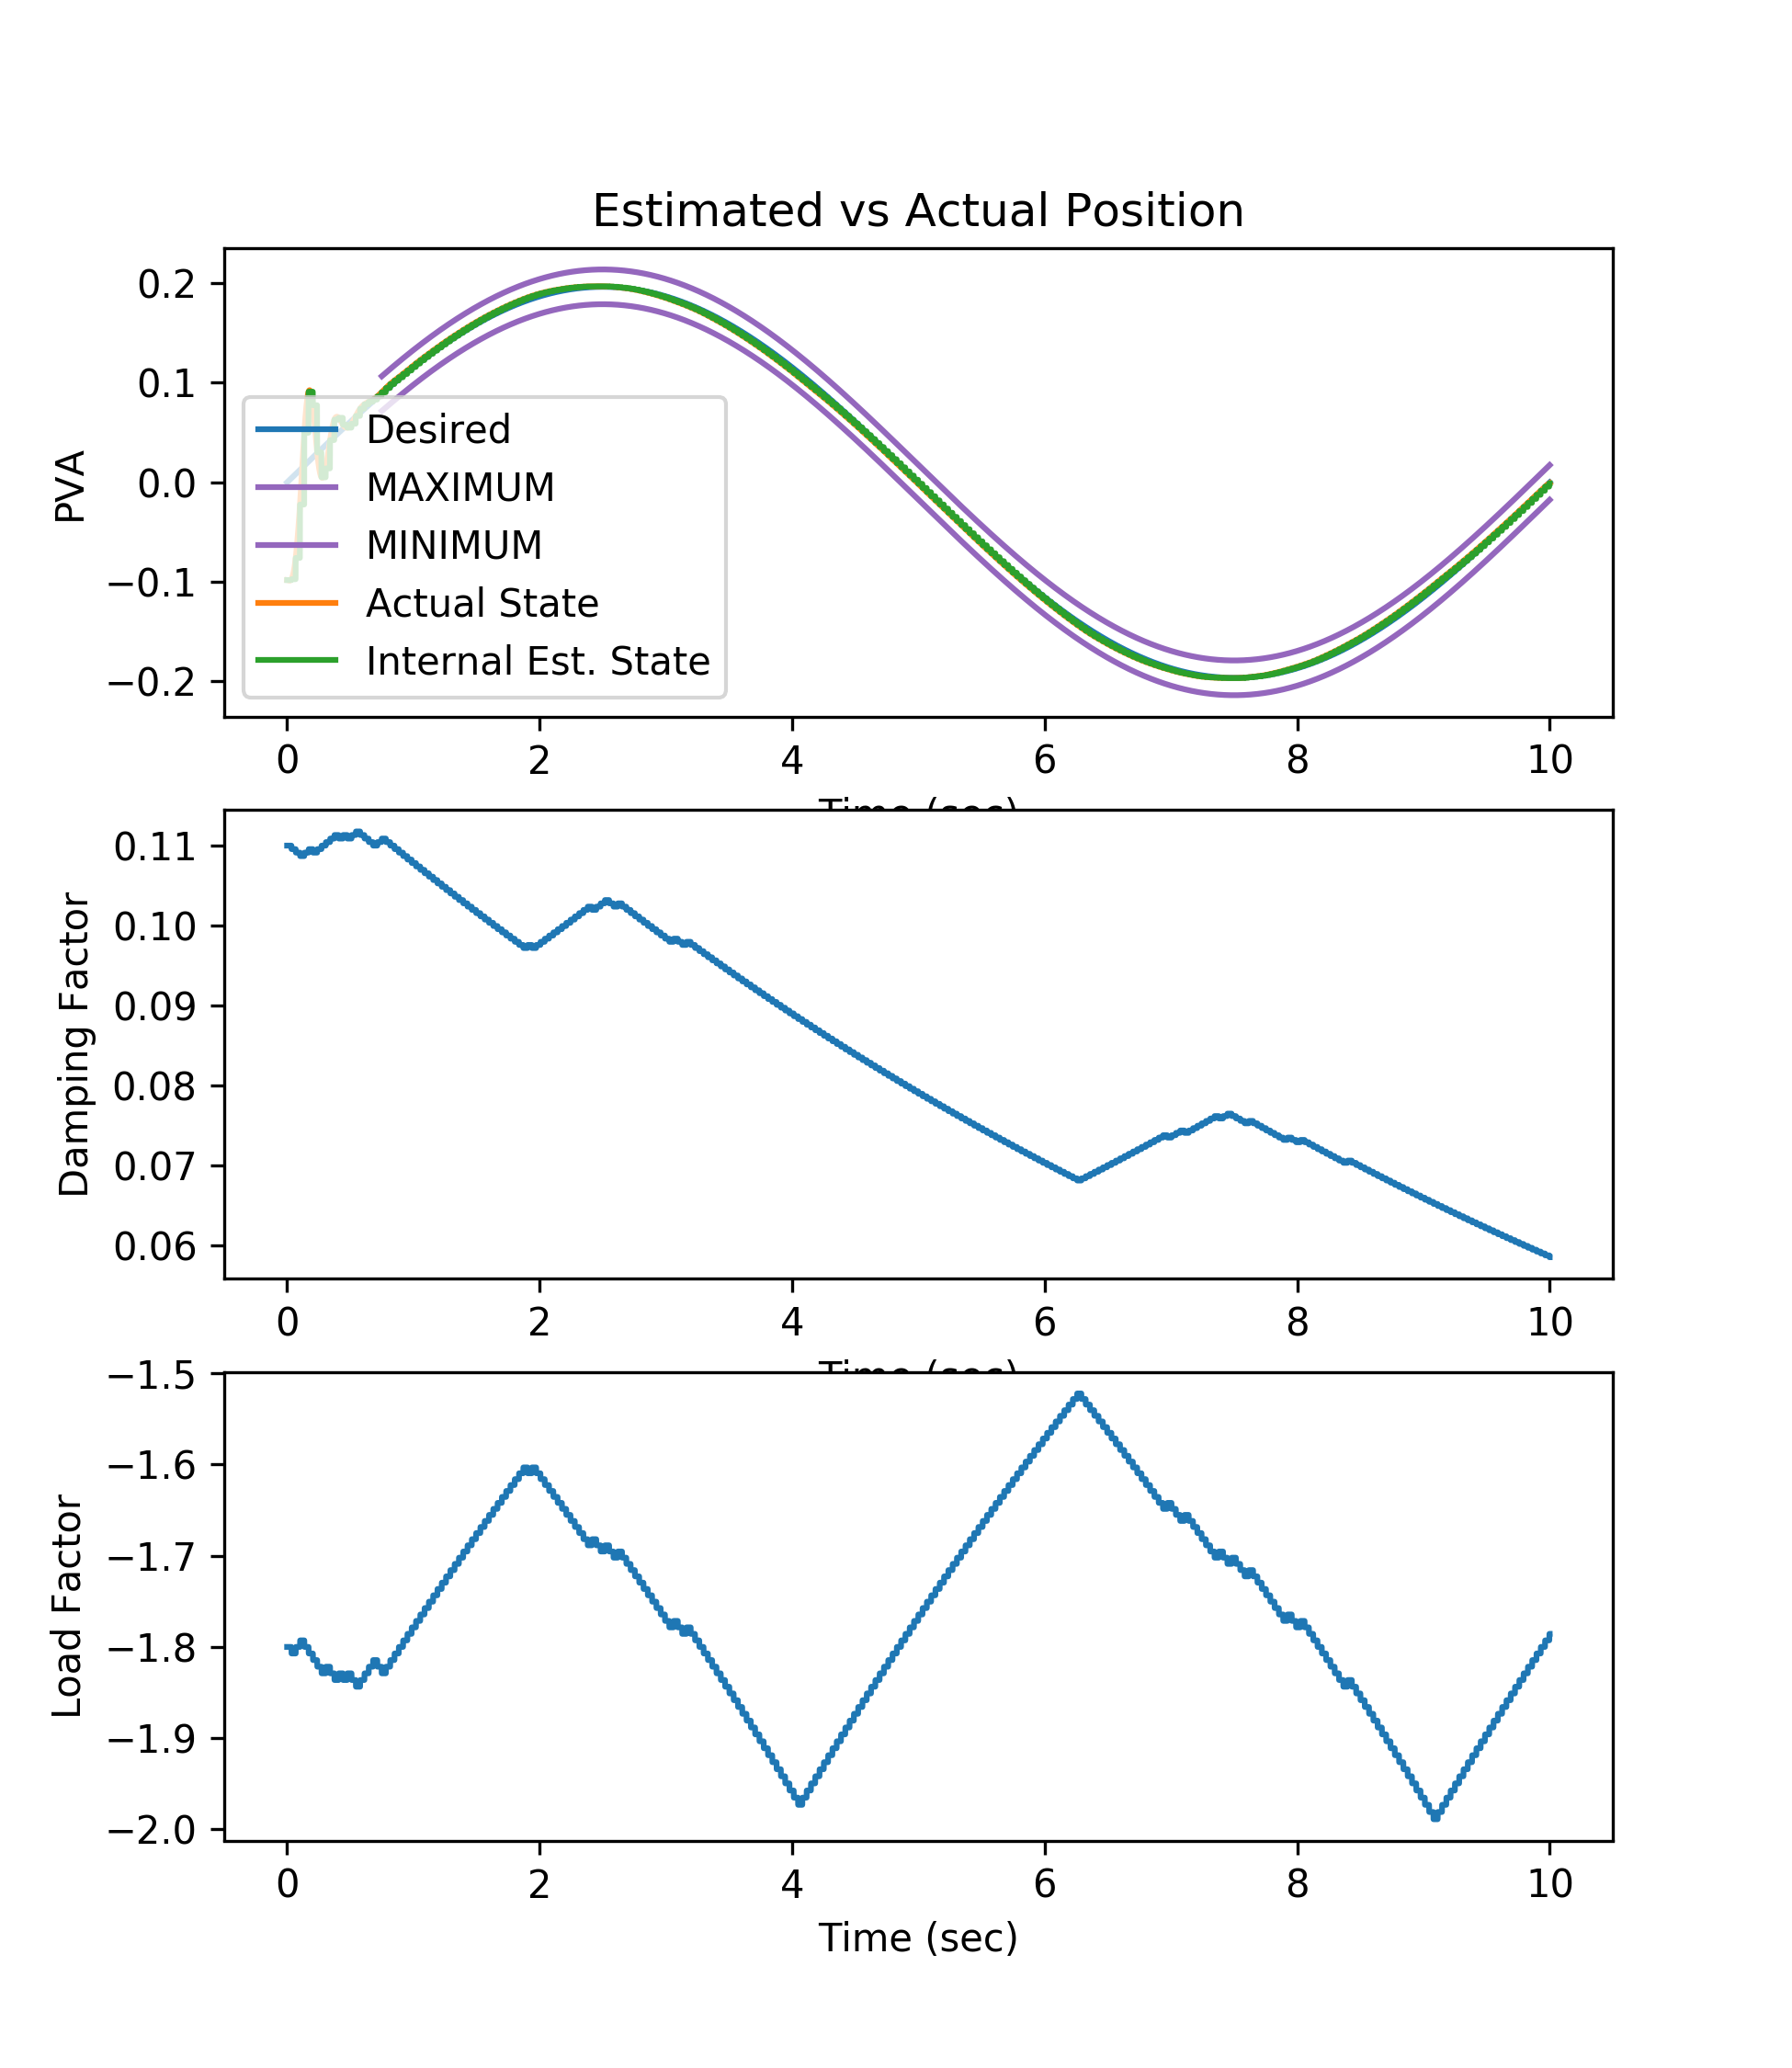
\includegraphics[height=7.5in]{results/State_Model_SimpleUpdate}
\caption{Successful tracking with simple parameter update}
\label{fig:StateUpdateSimple}
\end{figure}

\bbs{Neuron Controller}

Animatlab does not offer a good model of pneumatic muscles for use in closed loop testing. In place of this testing, the Python simulation was used to simulate the behavior of the pneumatic actuators and the neuron model was tuned to try and match the output of the Python controller from the small component subnetworks up to the overall controller behavior.

\bbss{Test Results}

Test results are generated based on data tools in \github{PuppyNeuronPlayground}. Post processing and visualization is done with scripts found in \github{writeup/scripts}.

\begin{figure}
\centering
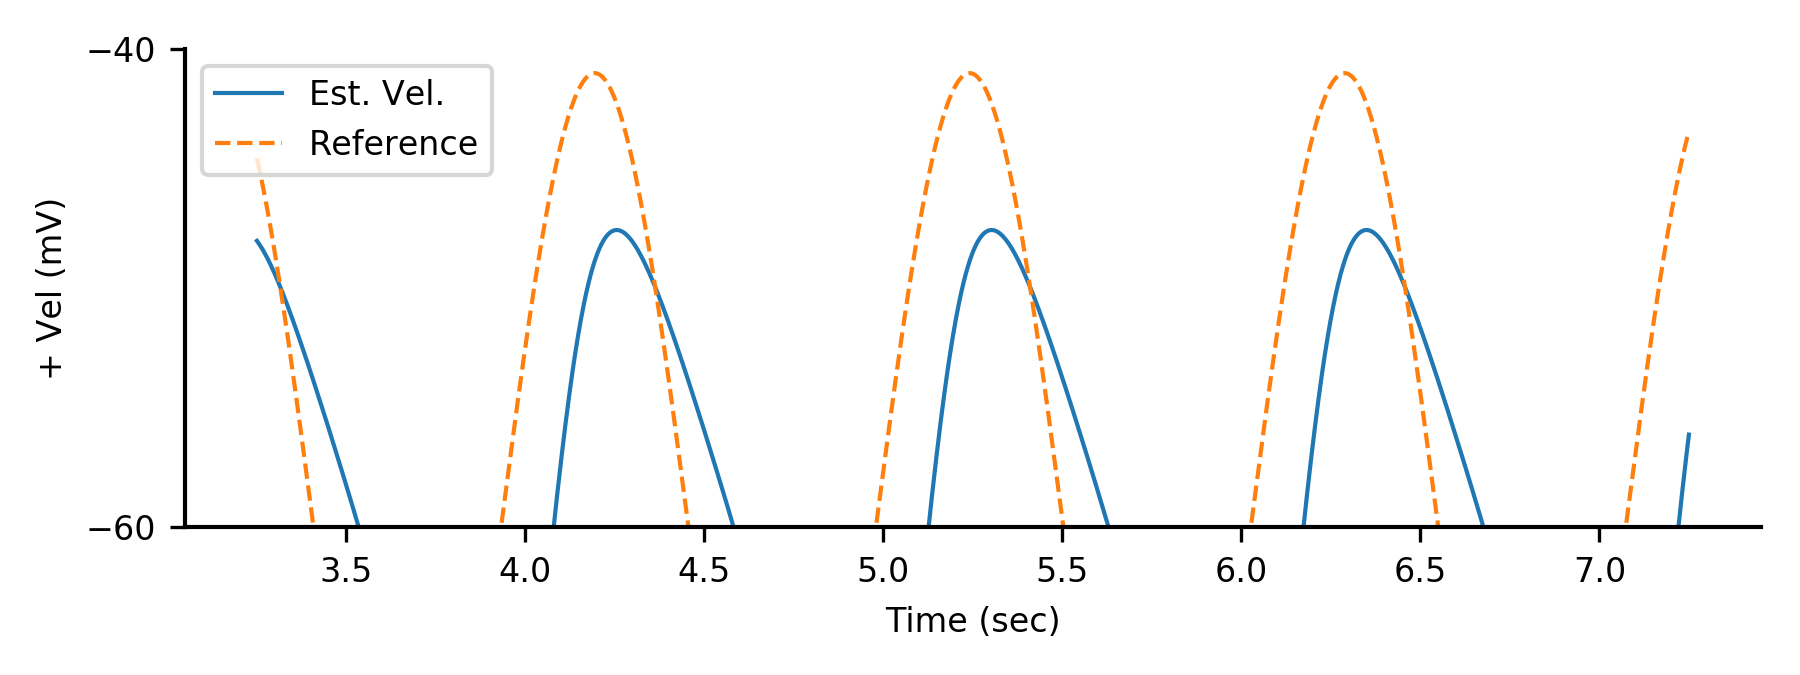
\includegraphics[height=2.25in]{results/TestVelPosWide}
\caption{Testing positive velocity estimation}
\label{fig:TestVelPos}
\end{figure}

\begin{figure}
\centering
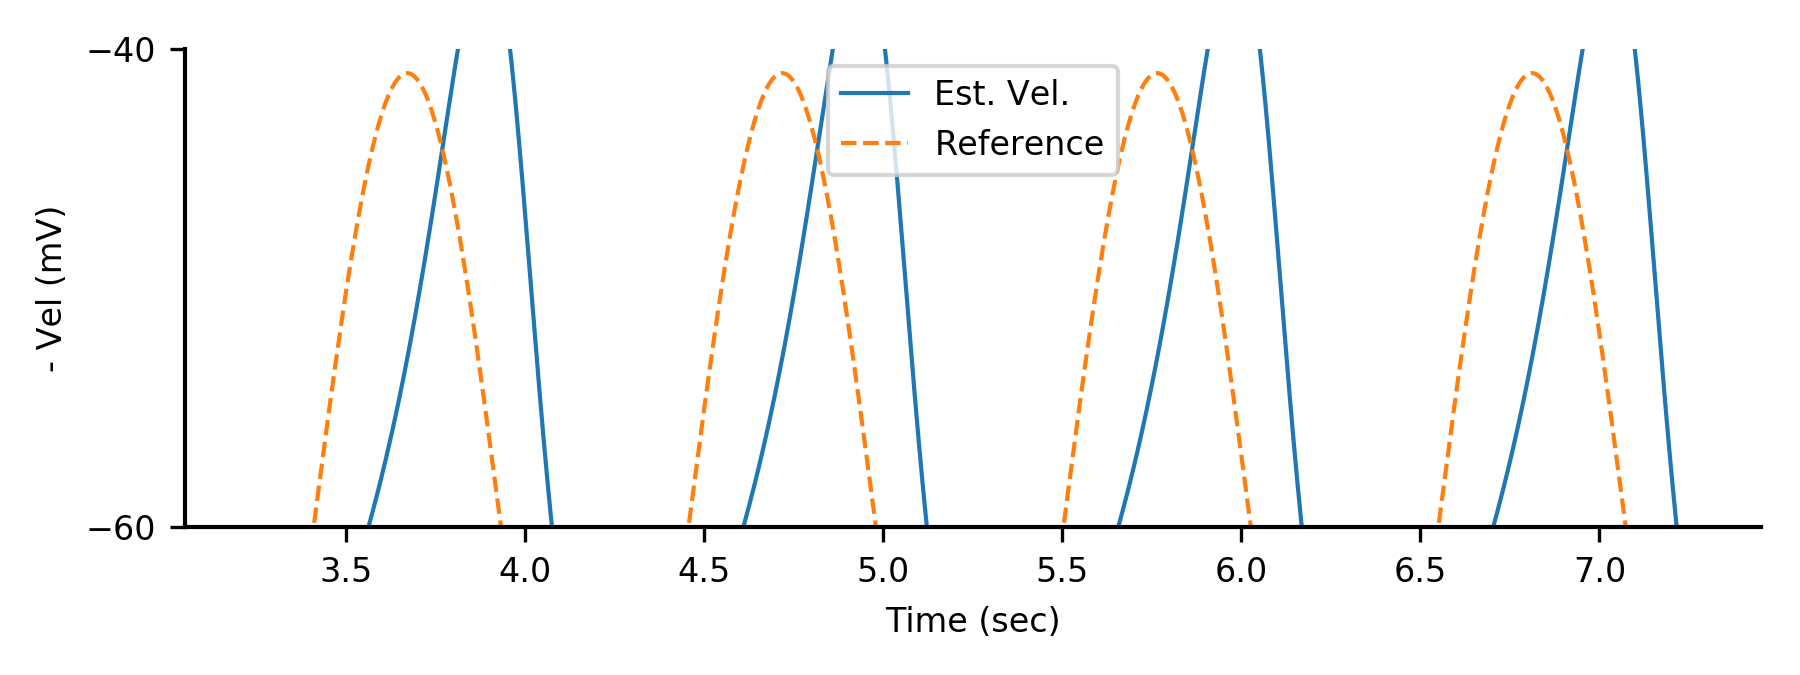
\includegraphics[height=2.25in]{results/TestVelNegWide}
\caption{Testing negative velocity estimation}
\label{fig:TestVelNeg}
\end{figure}

\begin{figure}
\centering
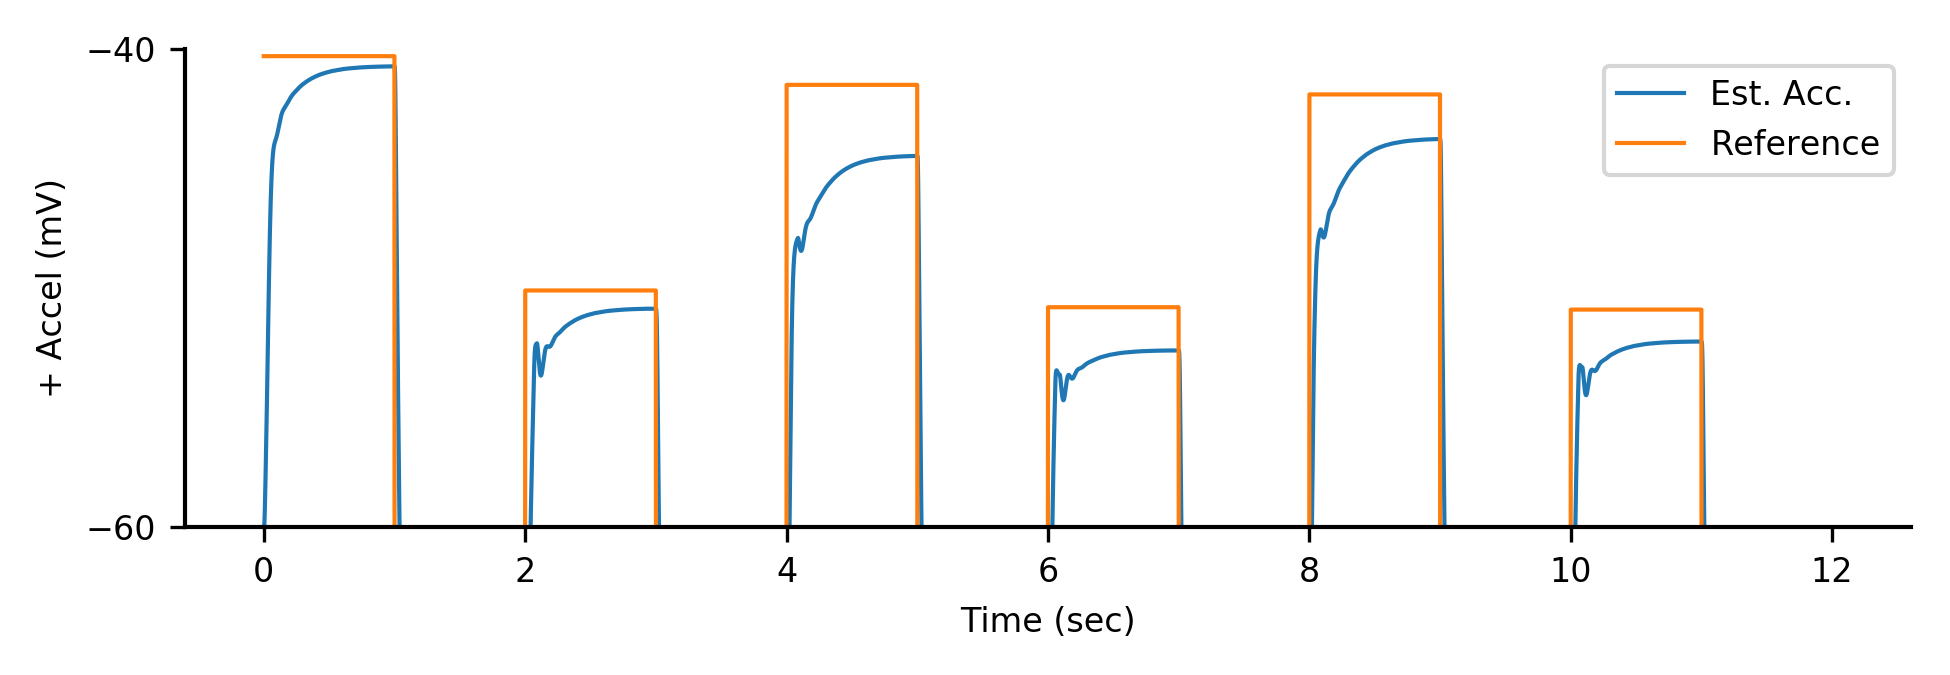
\includegraphics[height=2.25in]{results/TestAccelPosWide}
\caption{Testing positive acceleration estimation}
\label{fig:TestAccelPos}
\end{figure}

\begin{figure}
\centering
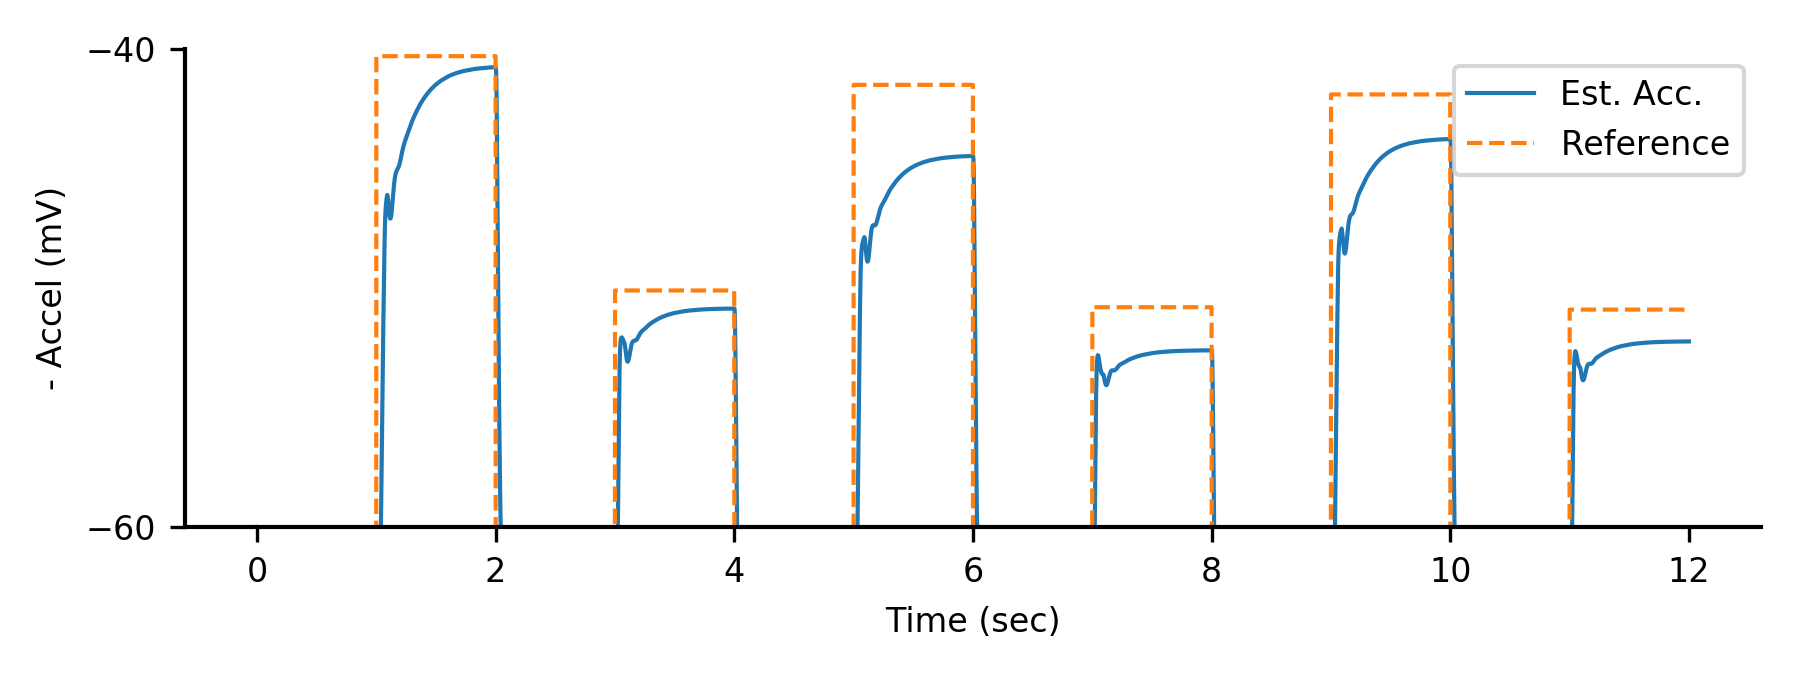
\includegraphics[height=2.25in]{results/TestAccelNegWide}
\caption{Testing negative acceleration estimation}
\label{fig:TestAccelNeg}
\end{figure}

\begin{figure}
\centering
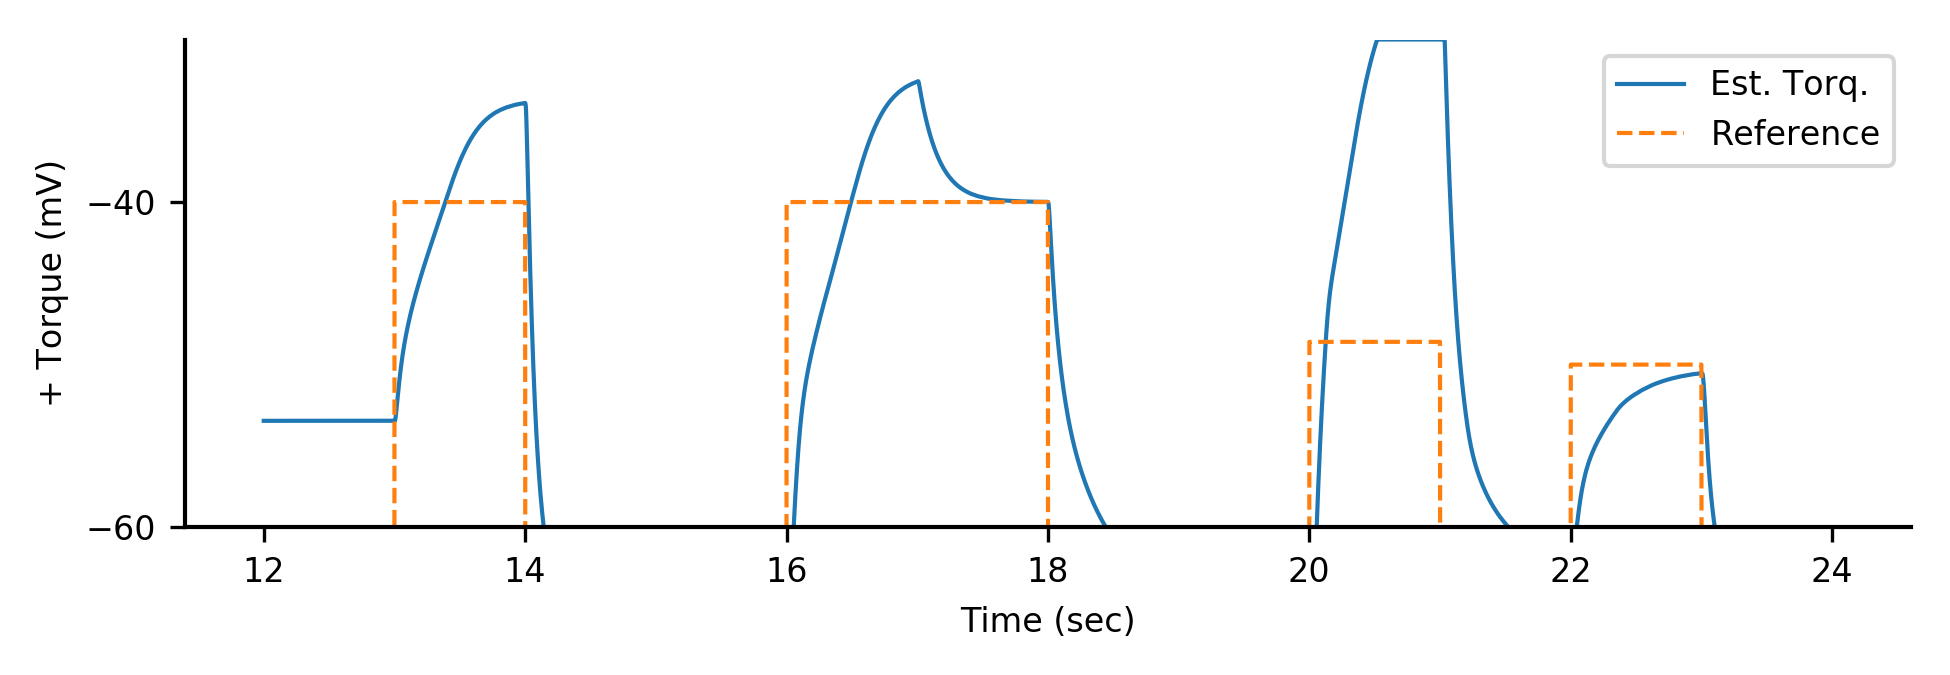
\includegraphics[height=2.25in]{results/TestTorqueOptimizationPosWide}
\caption{Testing positive torque optimization loop}
\label{fig:TestTorqueOptimizationPos}
\end{figure}

\begin{figure}
\centering
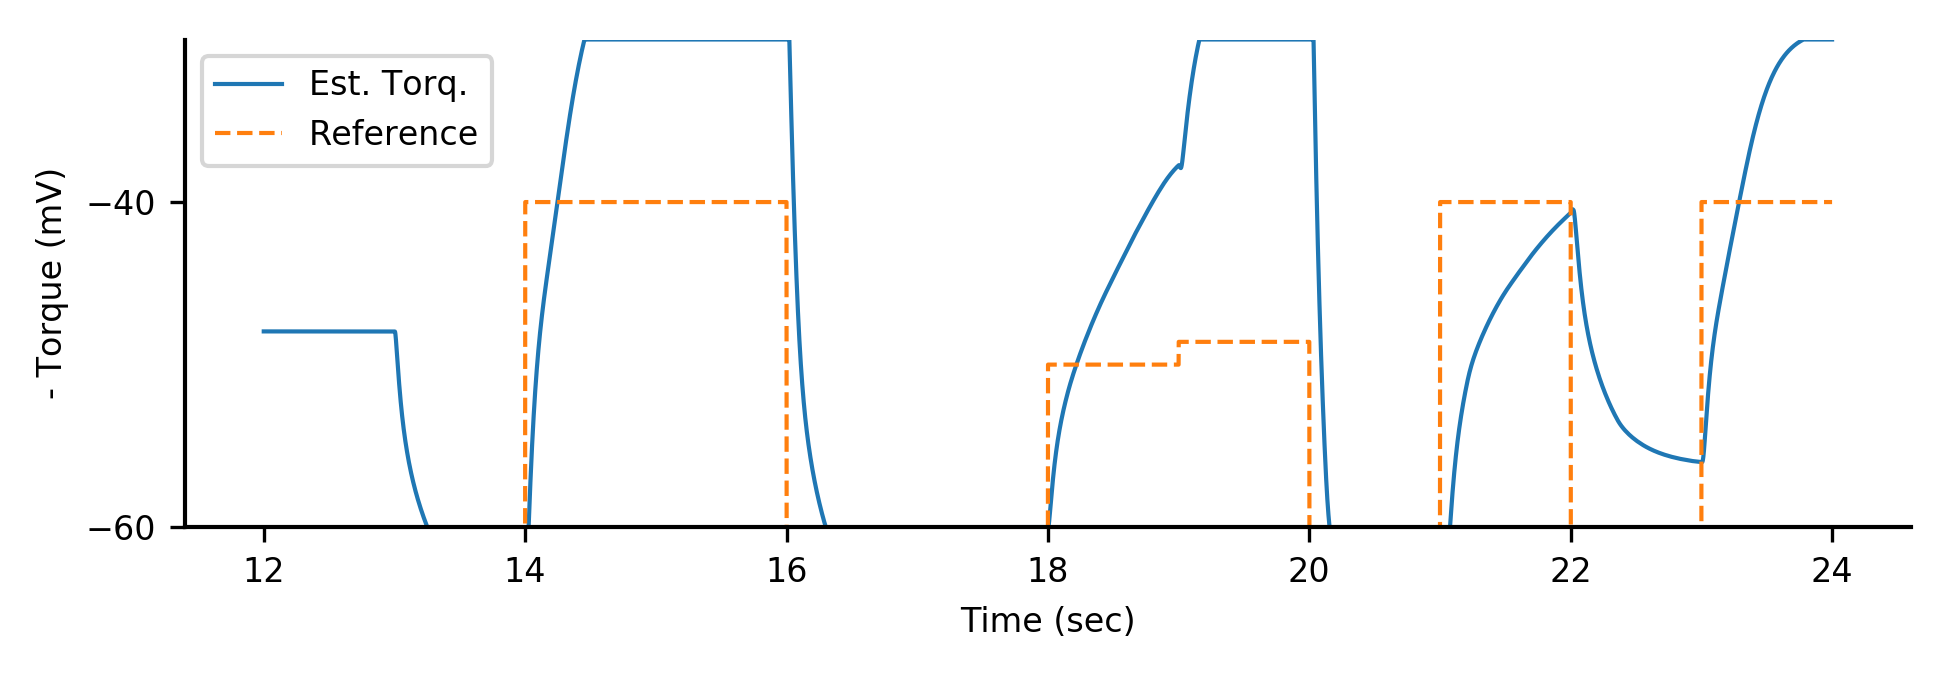
\includegraphics[height=2.25in]{results/TestTorqueOptimizationNegWide}
\caption{Testing negative torque optimization loop}
\label{fig:TestTorqueOptimizationNeg}
\end{figure}

\begin{figure}
\centering
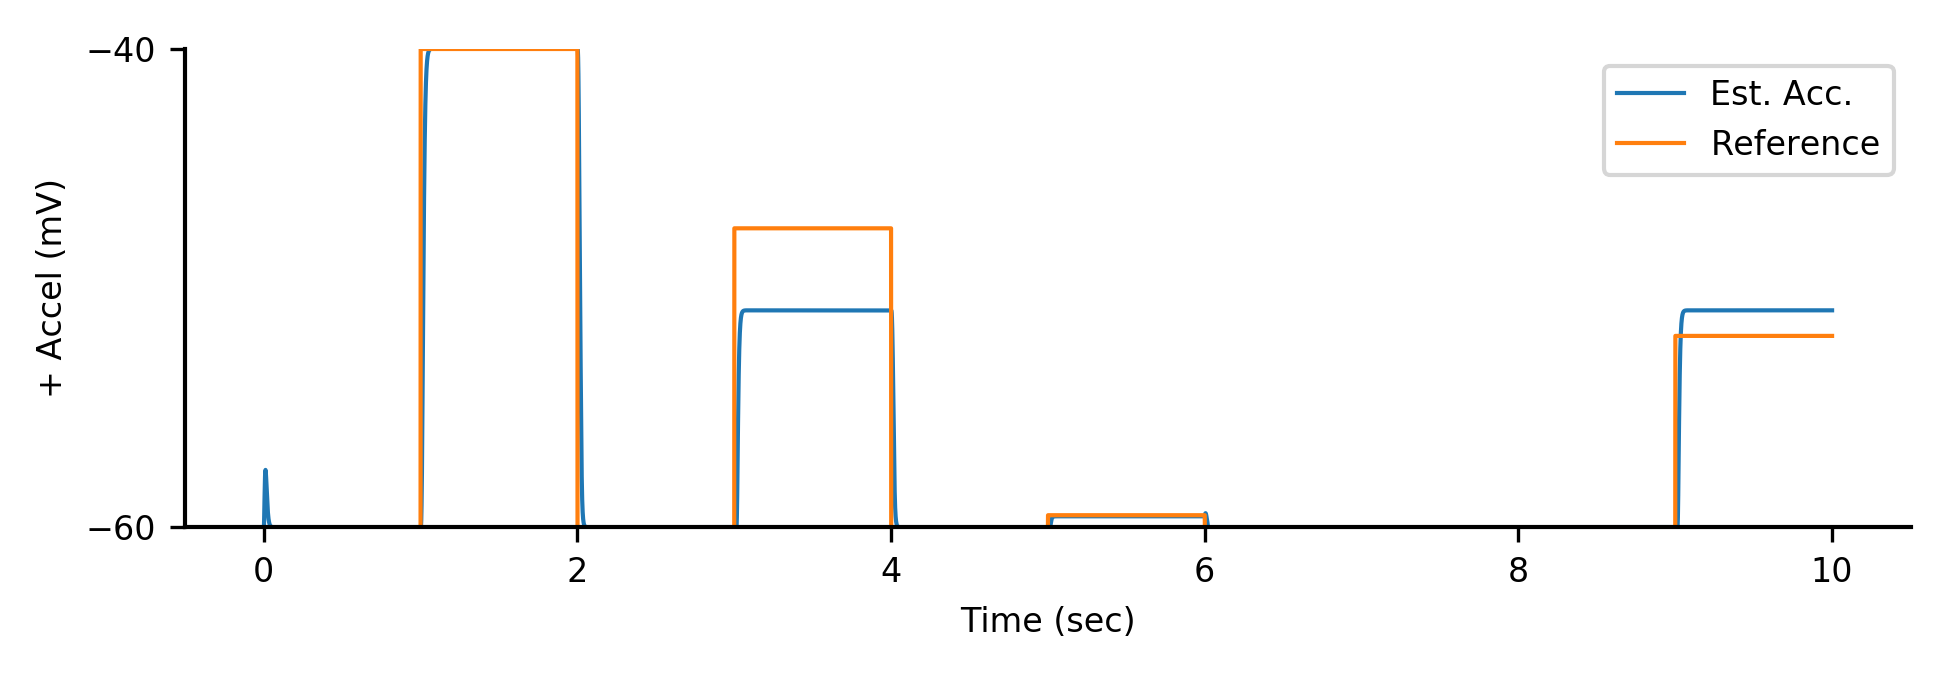
\includegraphics[height=2.25in]{results/TestT2APosWide}
\caption{Estimated positive acceleration from torque}
\label{fig:TestT2APos}
\end{figure}

\begin{figure}
\centering
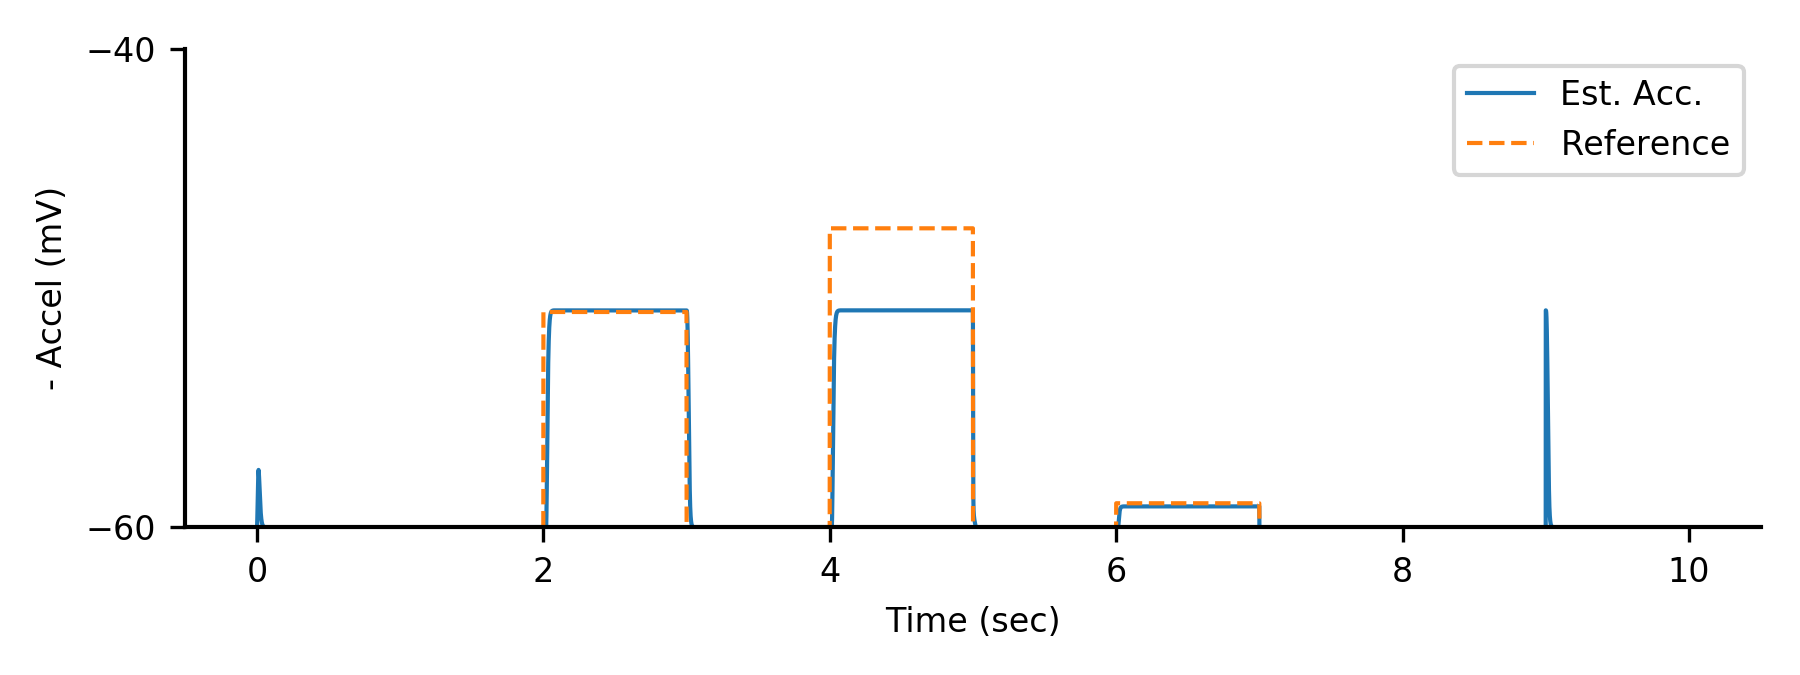
\includegraphics[height=2.25in]{results/TestT2ANegWide}
\caption{Estimated negative acceleration from torque}
\label{fig:TestT2ANeg}
\end{figure}

\begin{figure}
\centering
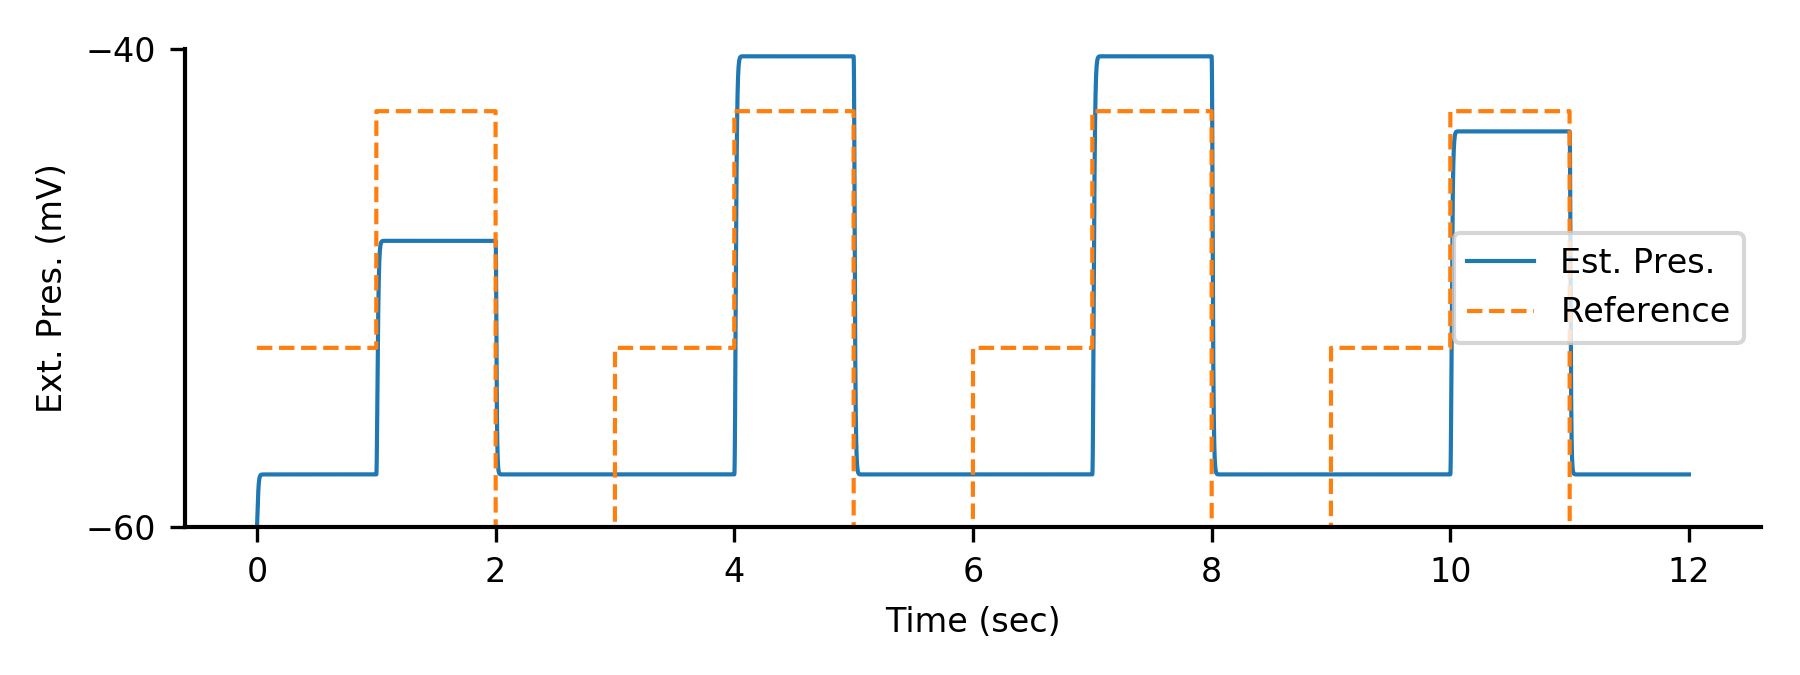
\includegraphics[height=2.25in]{results/TestT2PExtWide}
\caption{Estimated extension pressure from desired torque}
\label{fig:TestT2PPos}
\end{figure}

\begin{figure}
\centering
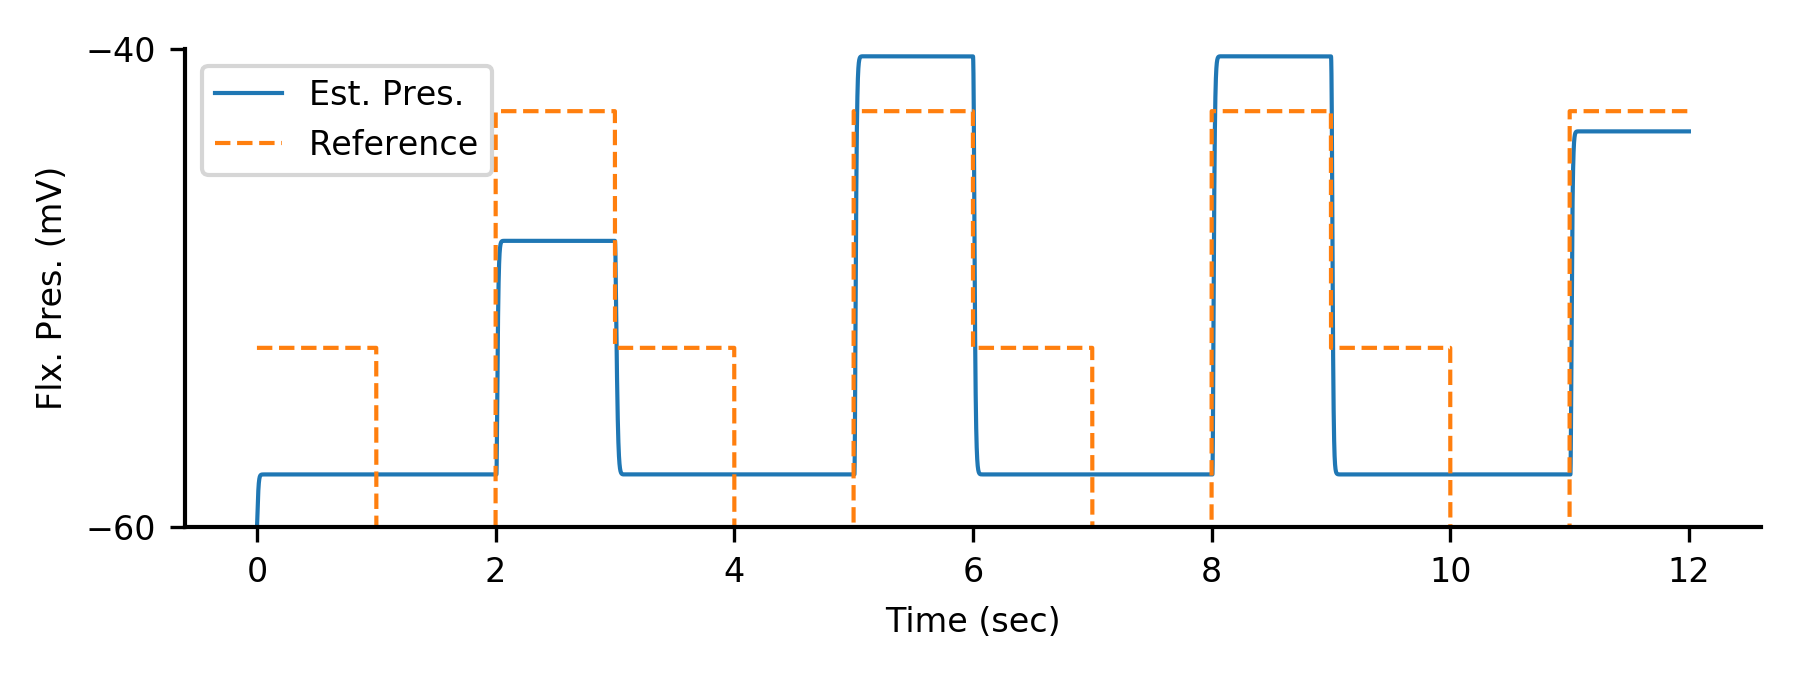
\includegraphics[height=2.25in]{results/TestT2PFlxWide}
\caption{Estimated flexion pressure from desired torque}
\label{fig:TestT2PNeg}
\end{figure}

\begin{figure}
\centering
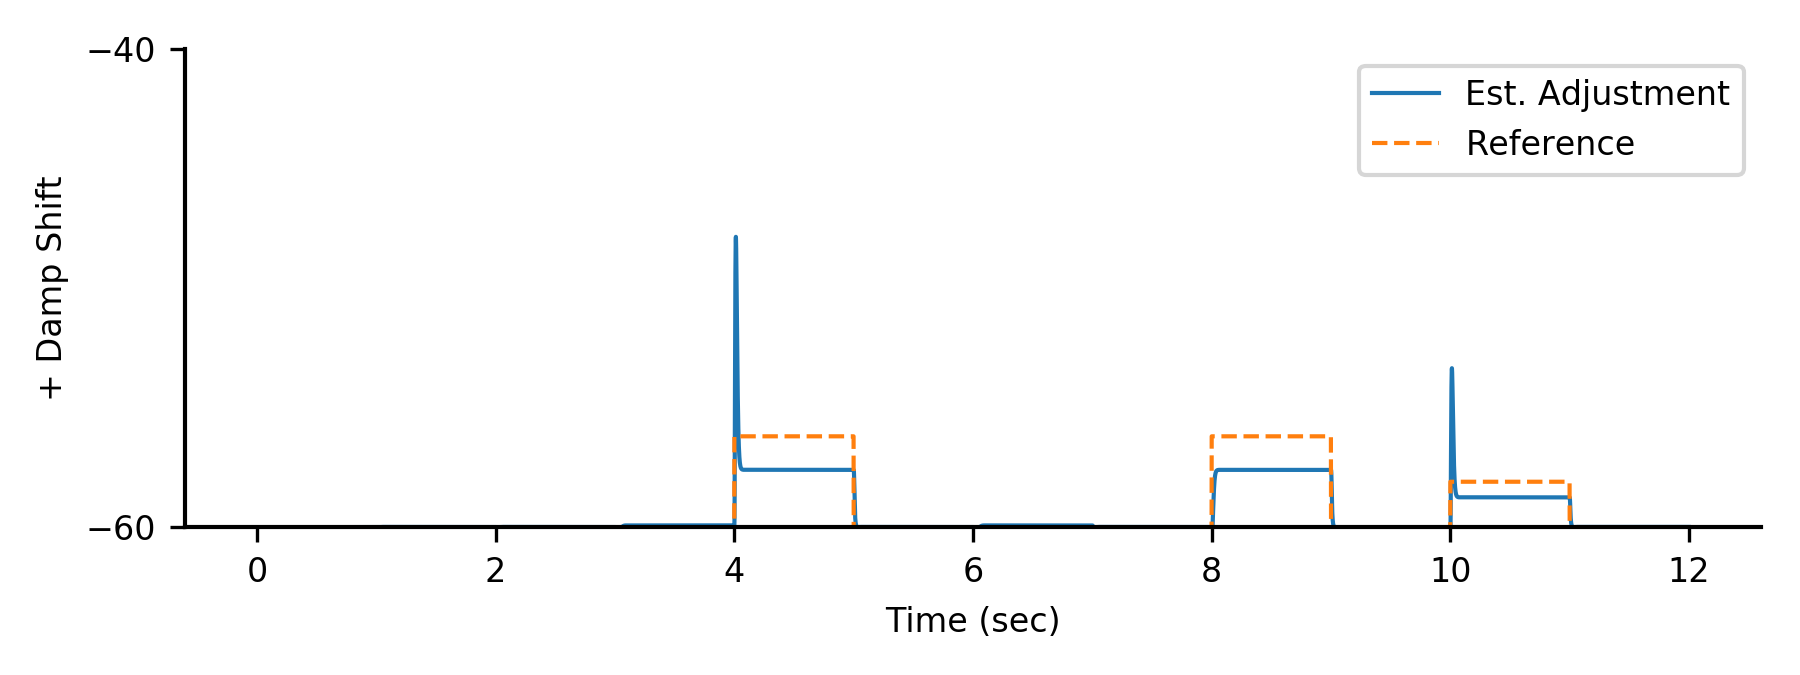
\includegraphics[height=2.25in]{results/TestSystemCPosWide}
\caption{Positive neuron and actual damping factor updates}
\label{fig:TestSystemCPos}
\end{figure}

\begin{figure}
\centering
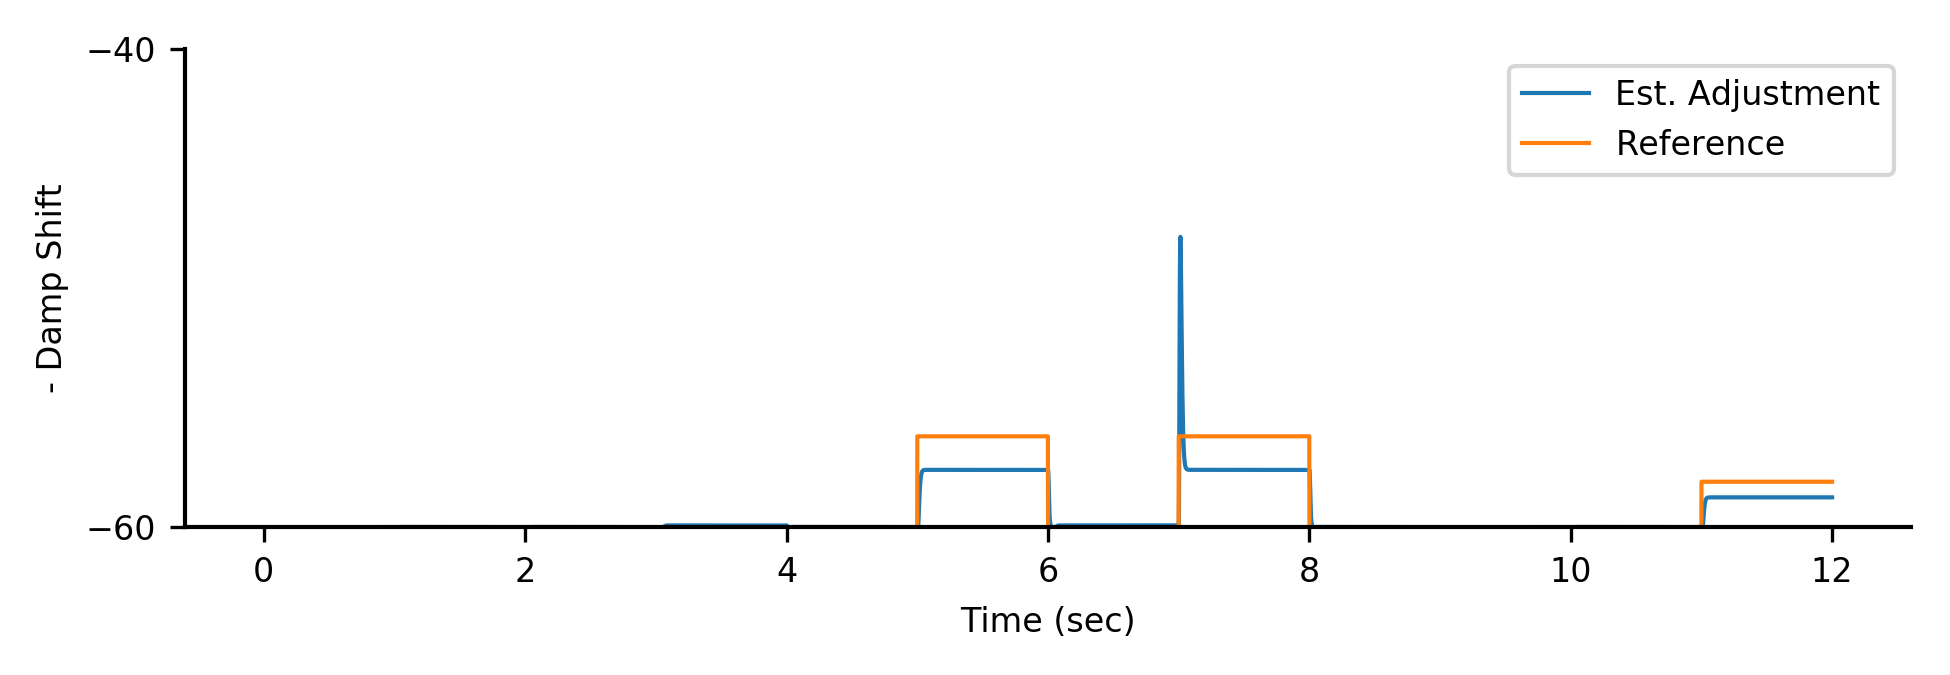
\includegraphics[height=2.25in]{results/TestSystemCNegWide}
\caption{Negative neuron and actual damping factor updates}
\label{fig:TestSystemCNeg}
\end{figure}

\begin{figure}
\centering
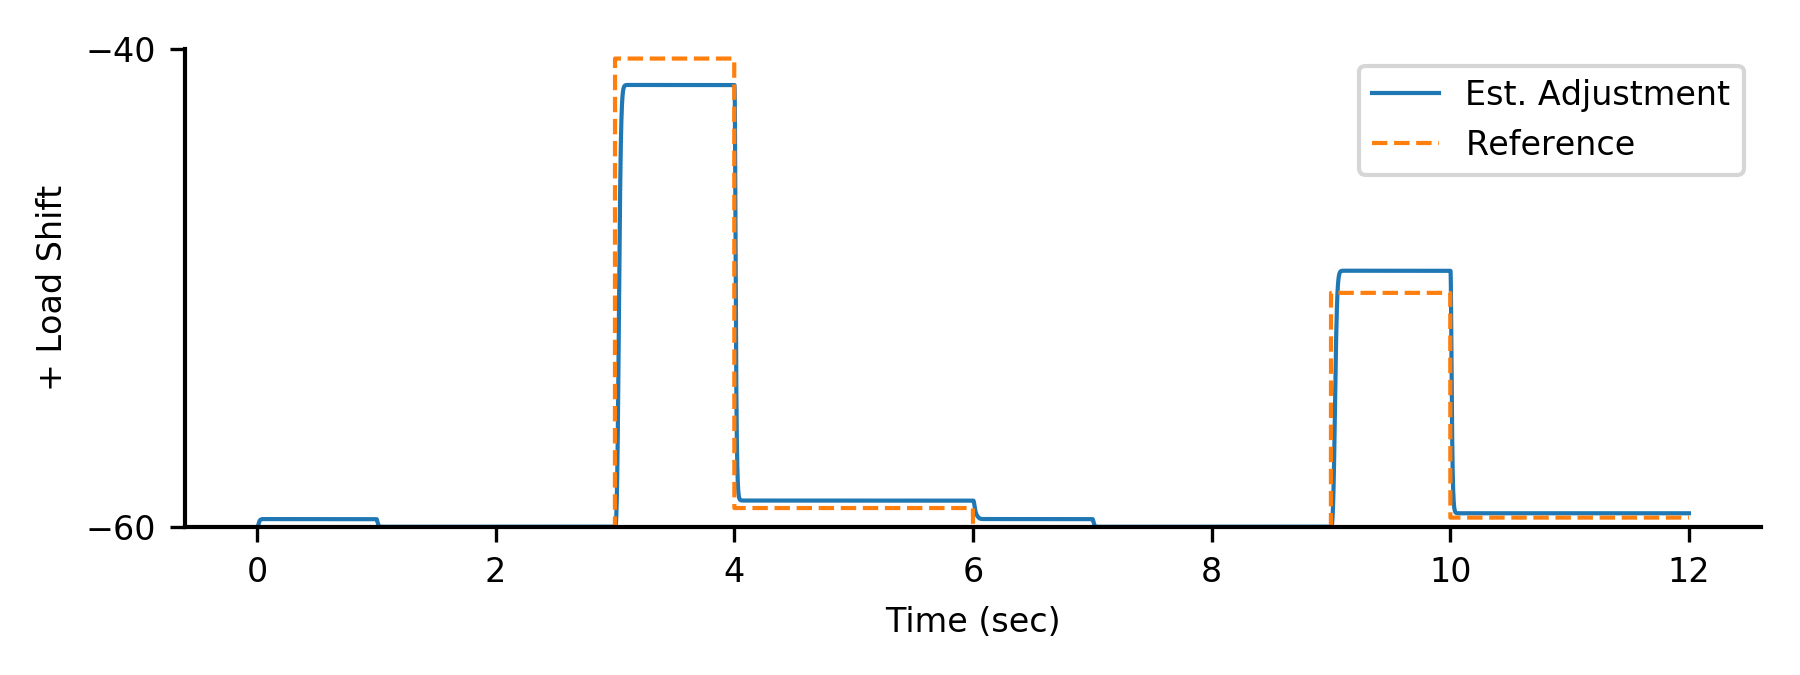
\includegraphics[height=2.25in]{results/TestSystemNPosWide}
\caption{Positive neuron and actual load factor updates}
\label{fig:TestSystemNPos}
\end{figure}

\begin{figure}
\centering
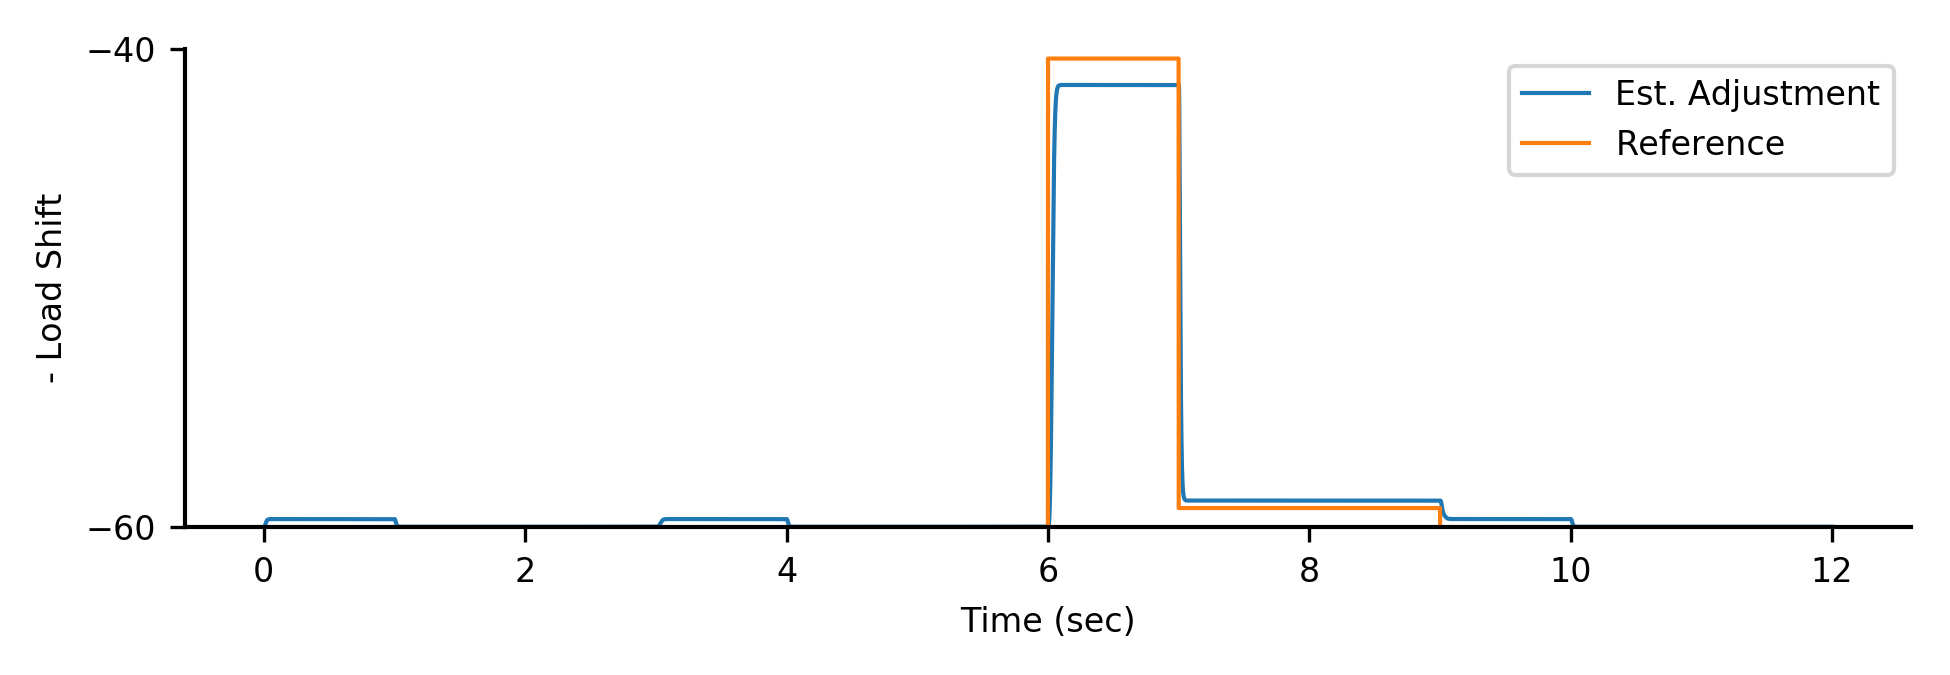
\includegraphics[height=2.25in]{results/TestSystemNNegWide}
\caption{Negative neuron and actual load factor updates}
\label{fig:TestSystemNNeg}
\end{figure}

\bbsss{Sensor Fusion}

Two key estimates are made within the sensor fusion subnetwork: velocity and
acceleration. The synthetic nervous system controller was tested against sine waves of known
frequencies. The positive and negative estimated are compared to the ground truth in \myref{fig:TestVelPos} and \myref{fig:TestVelNeg}.
Within the neuron network, acceleration is calculated primarily from actuator
pressures. The output is plotted compared with expected output. See
\myref{fig:TestAccelPos} and \myref{fig:TestAccelNeg}.

\bbsss{Torque Optimization}

The torque optimization network was tested as a complete network. Taking the entire network as a whole, the inputs (position, velocity and desired position) are driven to input values and the outputs are compared with the torque predictions of the prototype controller. In the same way that unit tests may not catch all types of software bugs, this kind of higher level test is designed to comprehensively test the connectivity between smaller subnetworks examined in other tests. The results of the tests are shown in \myref{fig:TestTorqueOptimizationPos} and \myref{fig:TestTorqueOptimizationNeg}.
The components for converting the torque to
acceleration also were tested
separately. See \myref{fig:TestT2APos} and \myref{fig:TestT2ANeg}.
The components for converting the torque to pressure also were tested
separately. See \myref{fig:TestT2PPos} and \myref{fig:TestT2PNeg}.

\bbss{System Modeling}

The system modeling network was tested as a complete network because both the
damping and load factors are updated from the same $\lambda$ value. See 
\myref{fig:TestSystemCPos}, \myref{fig:TestSystemCNeg},
\myref{fig:TestSystemNPos} and \myref{fig:TestSystemNNeg}.

\bbss{Discussion}
\label{chap:discussion}

In this thesis, we propose a new system for controlling joints actuated with
pneumatic artificial muscles. The design focuses on improving controller
performance through improved sensor processing, an internal optimization step
and an observer that continually updates the internal physics model to improve
the optimization step. This design was implemented as part of a synthetic
nervous system controller, with modifications made to the initial design to aid
in conversion to a neuron and synapse model and to take advantage of the benefits of the
synthetic nervous system approach.

\bbsss{Sensor Fusion}
\bbssss{Velocity}

The velocity network in the sensor fusion algorithm varies the most from the
reference data (see \myref{fig:TestVelPos} and \myref{fig:TestVelNeg}). This is a known phenomena addressed in
\cite{NickFunctionalSubnetwork}. This variance is observed in two quantities,
the phase shift and the magnitude.

In the velocity network, the magnitude of the positive and negative
velocities varied quite widely compared with the reference, especially at
higher gains. During the tuning of the network, a balance was chosen between
the maximum phase lag, minimized by decreasing the time constant of the slower
neuron, and increasing the synaptic gain (and therefore the observed difference between
positive and negative velocities).

This error suggests that there is an underlying error in the way that positive
and negative operations are computed; however, through individual tuning the
synapses appear to be relatively accurate. The use of the derivative network
varies in each application across different subnetworks. The engineering
solution for the correct balance of accuracy, gain and phase varies. This
variance leaves open the opportunity for biology to inform a single true correct
solution or a more complex derivative network that can independently select for
gain and phase.

\bbssss{Acceleration}

The acceleration network converges to a near-correct solution.
This convergence demonstrates that the feedback loop concept can be effective; however, the process takes a relatively long, fixed amount of time to
converge from solutions that are a significant step away. This time delay may lead to
issues with rapidly changing pressures on a hardware system. One potential
solution is to modify the time constants of the network
elements within the loop, in particular the integration network, to allow the
internal loop(s) to run faster than the rest of the network
so the outputs of the internal loop appear to converge to the correct value on the same time scale as the
rest of the network.

% TODO(buckbaskin): Cite Nick's leg-local mechanisms paper that (reaches the same conclusion?)

\bbsss{Torque Optimization}

In many cases the torque optimization network converges to the
correct solution; however, like the feedback in the acceleration network, the torque optimization process can
take a relatively long time to converge to the correct solution from discontinuous starting
values. Due to the integrator included in the torque optimization network, the starting conditions
for the first test case are based on other tests and did not show consistent
behavior.

The concept of the torque optimization network appears to be effective; however,
its implementation in neurons suffers from both attempting to converge to a
solution quickly and approximating a physical simulation internally. The torque optimization network
uses relatively low time constants and high gains. This can cause overshoot
(seen in \myref{fig:TestTorqueOptimizationPos}) where the
estimated torque is off the charts for either large positive or negative swings.
The high gains also reduce accuracy by amplifying small errors made during the
approximation of the ``physics" implementation. This behavior replicates
observations made during the development of the prototype controller in code,
where an attempt to approximate the physics of the joint in a single step was
inaccurate. The solution to the simulation error was to make multiple iterations by subdividing
the simulated time so that a simpler physics model would have a closer fit to
the actual dynamics. The iteration in the prototype controller suggests that a longer string of neurons would be
necessary within the loop to project dynamics forward; however, increasing the length of the feedback loop may accentuate existing delays when interfaced to hardware.

\bbssss{Acceleration from Torque}

The 3 stage network for estimating the acceleration from the torque applied to
the system appears to work well. There are two test cases, between 7 and 9
seconds that were not significant when tested at the resolution that the
network incorporates (shown in \myref{TestT2APos} and \myref{TestT2ANeg}). Otherwise, the acceleration is almost always correct.
Given its intended uses, the network is sufficiently accurate and suggests that
relatively small sets of neurons can provide a representation of the physics of
a biological system. This would suggest that an animal's nervous system can understand the dynamics of its environment and its body.

\bbssss{Estimating Pressures from Torques}

The process for calculating pressures from torques is accurate in some
cases and inaccurate in many others. This varying accuracy suggests that the physical
model of the pneumatic artificial muscles proposed in \cite{HuntPMuscles}
does not convert well to a relatively small network of neurons. A future controller iteration may elect to move the
calculation of this conversion out of neurons and
to LabView other other code used to interface between synthetic neurons and
hardware.

\bbsss{System Model}

The network for predicting the weight update is very accurate and suggests that
the engineered process of estimating the modeling errors of a synthetic neuron
network within the network itself is both feasible and an effective process for
the continual improvement of a controller applied to a particular hardware
joint under control.

This synthetic nervous system application also is generally more suitable to neuron networks than say,
the calculation of the conversion from pressures to torques following a well
prescribed algorithm involving a shifted tangent function. The exact magnitude
of the update of the weights, especially at a reduced gain, is not as important
as the relative magnitude and sign of each update. This characterisitic means that the
implementation of an arithmetic operation or dynamic calculation by a synapse of
a collection of synapses is tolerant to small variances from the expected
behavior.


\chapter{Conclusions and Future Work}
\label{chap:conclusion}
\bbs{Conclusion}

This thesis presents the design of a new style of biologically inspired
controller for controlling revolute joints with antagonistic pneumatic
artificial muscles. First, the literature surrounding the characterization of
the actuators and the methods used to control them is discussed in
\myref{chap:lit_review}. Second, the
design of a prototype for a controller is discussed in
\myref{chap:controller_design}. Third, the implementation of the design in a
synthetic nervous system is discussed in \myref{chap:neuron_design}. The methods
for testing the controller are discussed in \myref{chap:methods}. The results of
the tests are presented in \myref{chap:results}.

The controller implements new features not previously used in synthetic nervous
system design and not previously used for control of joints actuated by
pneumatic artificial muscles. The system has a whole has been shown to offer
increased accuracy in joint position and decreased phase shift. This was
combined with a better internal model of the actuators themselves to more
accurately model the forces and torques applied in order to continue successful
operation even near the maximum output of the actuators. On the other hand, the
successful operation of the controller is dependent on the tuning of a number of
internal parameters that are sensitive to slight overestimates that lead to
oscillation and loss of control of the joint. This has been mitigated by
asymmetric model updates that favor stable error and starting from known stable
estimates; however, this leads to tracking that does not meet the accuracy goals
discussed in the design when the parameters are too conservative.

The implementation of the controller in a synthetic nervous system led to the
design of unique nervous system functional subnetworks; however, some networks
were found to be inconsistent with their standard controller output, leading to
potential deficiencies in observed performance. This would suggest that a more
bionic approach that leverages mathematical models directly for complicated
calculations, such as the relation between pressure and torque for pneumatic
artificial muscles, and the dynamic benefits of a synthetic nervous system for
aspects of the controller that require less precision and benefit from insights
gained from a deeper biological understanding of how animal nervous systems
control joints.

\bbs{Future Work}

The next step for the design of the controller is experimental testing to
characterize performance on actual hardware. During simulation and testing,
many aspects of the controller worked well; on the other hand, some did not
behave as well as expected. On hardware, there is always some variation that may
show that the design choices made were effective and practical solutions.

There is also some potential for improvement of the design of the controller.
Further analysis of the stability of the controller may lead to a better model
update procedure. In particular, algorithms such as an Extended Kalman Filter
are used in many applications across robotics for estimating parameters from
sensor data; however, the Kalman Filter algorithm was not used because the matrix math operations (including an inversion) do
not have a good parallel implementation within a synthetic nervous system.
New biological research % TODO(buckbaskin): cite that paper with the toroid structure
suggests that animals have groups of neurons that estimate orientation and
% TODO(buckbaskin): and that time and space cells paper thing I found
position in time and space. This research suggests potential approximations for
spatial estimation that may be useful for estimation of other parameters to
emulate or replace the use of a Kalman Filter.

Another area where the neuron controller has room for improvement is
implementation of certain subnetworks that don't effectively implement their
counterparts in the prototype. There were approximations made to match neuron
and synapse behavior at a low level to some of the mathematics; however, taking
a larger system approach with an aim to design neuron connections to emulate
behavior of larger pieces of the system made lead to a more successful design.
The end goal is to design a working controller with similar properties, this
doesn't need to be achieved by direct copying. The testing methods implemented
in this thesis offer a good system for iterating on this kind of design. Test
inputs can be set up once and then higher level component behavior can be
compared quickly and visually.

Overall, the design of the controller presents a new style of design that can be
used to create optimal controllers for actuation systems that are highly
non-linear and tend to perform poorly when simpler controller designs are used.
There is room for improvement, but the methods used in the thesis offer a
framework for improvement and determining the areas with the largest impact.


\newpage
\label{chap:references}
%TODO(buckbaskin): clean out extra unnecessary information from references.bib
\printbibliography[heading=bibintoc, title={Bibliography}]

% \newpage
% \appendix
% \crefalias{section}{appsec}
% \chapter{Network Topology}
% \label{app:network_topologies}
% The code and configuration files for this project are available on Github at \url{https://github.com/buckbaskin/animatlab}.

% \chapter{Neuron Tests}
% \label{app:neuron_tests}
% Content!!

% TODO(buckbaskin): Insert an exhaustive list of the tested subnetworks here

Also, indicate which ones are unit networks and which are integration tests


\end{document}
